\documentclass[journal]{IEEEtran}
% IEEE two-column journal layout (IEEEtran v1.8b), prepared for IEEE J-BHI.
\usepackage[OT1]{fontenc}
%%%%% NEW MATH DEFINITIONS %%%%%

\usepackage{amsmath,amsfonts,bm}

% Mark sections of captions for referring to divisions of figures
\newcommand{\figleft}{{\em (Left)}}
\newcommand{\figcenter}{{\em (Center)}}
\newcommand{\figright}{{\em (Right)}}
\newcommand{\figtop}{{\em (Top)}}
\newcommand{\figbottom}{{\em (Bottom)}}
\newcommand{\captiona}{{\em (a)}}
\newcommand{\captionb}{{\em (b)}}
\newcommand{\captionc}{{\em (c)}}
\newcommand{\captiond}{{\em (d)}}

% Highlight a newly defined term
\newcommand{\newterm}[1]{{\bf #1}}


% Figure reference, lower-case.
\def\figref#1{figure~\ref{#1}}
% Figure reference, capital. For start of sentence
\def\Figref#1{Figure~\ref{#1}}
\def\twofigref#1#2{figures \ref{#1} and \ref{#2}}
\def\quadfigref#1#2#3#4{figures \ref{#1}, \ref{#2}, \ref{#3} and \ref{#4}}
% Section reference, lower-case.
\def\secref#1{section~\ref{#1}}
% Section reference, capital.
\def\Secref#1{Section~\ref{#1}}
% Reference to two sections.
\def\twosecrefs#1#2{sections \ref{#1} and \ref{#2}}
% Reference to three sections.
\def\secrefs#1#2#3{sections \ref{#1}, \ref{#2} and \ref{#3}}
% Reference to an equation, lower-case.
\def\eqref#1{equation~\ref{#1}}
% Reference to an equation, upper case
\def\Eqref#1{Equation~\ref{#1}}
% A raw reference to an equation---avoid using if possible
\def\plaineqref#1{\ref{#1}}
% Reference to a chapter, lower-case.
\def\chapref#1{chapter~\ref{#1}}
% Reference to an equation, upper case.
\def\Chapref#1{Chapter~\ref{#1}}
% Reference to a range of chapters
\def\rangechapref#1#2{chapters\ref{#1}--\ref{#2}}
% Reference to an algorithm, lower-case.
\def\algref#1{algorithm~\ref{#1}}
% Reference to an algorithm, upper case.
\def\Algref#1{Algorithm~\ref{#1}}
\def\twoalgref#1#2{algorithms \ref{#1} and \ref{#2}}
\def\Twoalgref#1#2{Algorithms \ref{#1} and \ref{#2}}
% Reference to a part, lower case
\def\partref#1{part~\ref{#1}}
% Reference to a part, upper case
\def\Partref#1{Part~\ref{#1}}
\def\twopartref#1#2{parts \ref{#1} and \ref{#2}}

\def\ceil#1{\lceil #1 \rceil}
\def\floor#1{\lfloor #1 \rfloor}
\def\1{\bm{1}}
\newcommand{\train}{\mathcal{D}}
\newcommand{\valid}{\mathcal{D_{\mathrm{valid}}}}
\newcommand{\test}{\mathcal{D_{\mathrm{test}}}}

\def\eps{{\epsilon}}


% Random variables
\def\reta{{\textnormal{$\eta$}}}
\def\ra{{\textnormal{a}}}
\def\rb{{\textnormal{b}}}
\def\rc{{\textnormal{c}}}
\def\rd{{\textnormal{d}}}
\def\re{{\textnormal{e}}}
\def\rf{{\textnormal{f}}}
\def\rg{{\textnormal{g}}}
\def\rh{{\textnormal{h}}}
\def\ri{{\textnormal{i}}}
\def\rj{{\textnormal{j}}}
\def\rk{{\textnormal{k}}}
\def\rl{{\textnormal{l}}}
% rm is already a command, just don't name any random variables m
\def\rn{{\textnormal{n}}}
\def\ro{{\textnormal{o}}}
\def\rp{{\textnormal{p}}}
\def\rq{{\textnormal{q}}}
\def\rr{{\textnormal{r}}}
\def\rs{{\textnormal{s}}}
\def\rt{{\textnormal{t}}}
\def\ru{{\textnormal{u}}}
\def\rv{{\textnormal{v}}}
\def\rw{{\textnormal{w}}}
\def\rx{{\textnormal{x}}}
\def\ry{{\textnormal{y}}}
\def\rz{{\textnormal{z}}}

% Random vectors
\def\rvepsilon{{\mathbf{\epsilon}}}
\def\rvtheta{{\mathbf{\theta}}}
\def\rva{{\mathbf{a}}}
\def\rvb{{\mathbf{b}}}
\def\rvc{{\mathbf{c}}}
\def\rvd{{\mathbf{d}}}
\def\rve{{\mathbf{e}}}
\def\rvf{{\mathbf{f}}}
\def\rvg{{\mathbf{g}}}
\def\rvh{{\mathbf{h}}}
\def\rvu{{\mathbf{i}}}
\def\rvj{{\mathbf{j}}}
\def\rvk{{\mathbf{k}}}
\def\rvl{{\mathbf{l}}}
\def\rvm{{\mathbf{m}}}
\def\rvn{{\mathbf{n}}}
\def\rvo{{\mathbf{o}}}
\def\rvp{{\mathbf{p}}}
\def\rvq{{\mathbf{q}}}
\def\rvr{{\mathbf{r}}}
\def\rvs{{\mathbf{s}}}
\def\rvt{{\mathbf{t}}}
\def\rvu{{\mathbf{u}}}
\def\rvv{{\mathbf{v}}}
\def\rvw{{\mathbf{w}}}
\def\rvx{{\mathbf{x}}}
\def\rvy{{\mathbf{y}}}
\def\rvz{{\mathbf{z}}}

% Elements of random vectors
\def\erva{{\textnormal{a}}}
\def\ervb{{\textnormal{b}}}
\def\ervc{{\textnormal{c}}}
\def\ervd{{\textnormal{d}}}
\def\erve{{\textnormal{e}}}
\def\ervf{{\textnormal{f}}}
\def\ervg{{\textnormal{g}}}
\def\ervh{{\textnormal{h}}}
\def\ervi{{\textnormal{i}}}
\def\ervj{{\textnormal{j}}}
\def\ervk{{\textnormal{k}}}
\def\ervl{{\textnormal{l}}}
\def\ervm{{\textnormal{m}}}
\def\ervn{{\textnormal{n}}}
\def\ervo{{\textnormal{o}}}
\def\ervp{{\textnormal{p}}}
\def\ervq{{\textnormal{q}}}
\def\ervr{{\textnormal{r}}}
\def\ervs{{\textnormal{s}}}
\def\ervt{{\textnormal{t}}}
\def\ervu{{\textnormal{u}}}
\def\ervv{{\textnormal{v}}}
\def\ervw{{\textnormal{w}}}
\def\ervx{{\textnormal{x}}}
\def\ervy{{\textnormal{y}}}
\def\ervz{{\textnormal{z}}}

% Random matrices
\def\rmA{{\mathbf{A}}}
\def\rmB{{\mathbf{B}}}
\def\rmC{{\mathbf{C}}}
\def\rmD{{\mathbf{D}}}
\def\rmE{{\mathbf{E}}}
\def\rmF{{\mathbf{F}}}
\def\rmG{{\mathbf{G}}}
\def\rmH{{\mathbf{H}}}
\def\rmI{{\mathbf{I}}}
\def\rmJ{{\mathbf{J}}}
\def\rmK{{\mathbf{K}}}
\def\rmL{{\mathbf{L}}}
\def\rmM{{\mathbf{M}}}
\def\rmN{{\mathbf{N}}}
\def\rmO{{\mathbf{O}}}
\def\rmP{{\mathbf{P}}}
\def\rmQ{{\mathbf{Q}}}
\def\rmR{{\mathbf{R}}}
\def\rmS{{\mathbf{S}}}
\def\rmT{{\mathbf{T}}}
\def\rmU{{\mathbf{U}}}
\def\rmV{{\mathbf{V}}}
\def\rmW{{\mathbf{W}}}
\def\rmX{{\mathbf{X}}}
\def\rmY{{\mathbf{Y}}}
\def\rmZ{{\mathbf{Z}}}

% Elements of random matrices
\def\ermA{{\textnormal{A}}}
\def\ermB{{\textnormal{B}}}
\def\ermC{{\textnormal{C}}}
\def\ermD{{\textnormal{D}}}
\def\ermE{{\textnormal{E}}}
\def\ermF{{\textnormal{F}}}
\def\ermG{{\textnormal{G}}}
\def\ermH{{\textnormal{H}}}
\def\ermI{{\textnormal{I}}}
\def\ermJ{{\textnormal{J}}}
\def\ermK{{\textnormal{K}}}
\def\ermL{{\textnormal{L}}}
\def\ermM{{\textnormal{M}}}
\def\ermN{{\textnormal{N}}}
\def\ermO{{\textnormal{O}}}
\def\ermP{{\textnormal{P}}}
\def\ermQ{{\textnormal{Q}}}
\def\ermR{{\textnormal{R}}}
\def\ermS{{\textnormal{S}}}
\def\ermT{{\textnormal{T}}}
\def\ermU{{\textnormal{U}}}
\def\ermV{{\textnormal{V}}}
\def\ermW{{\textnormal{W}}}
\def\ermX{{\textnormal{X}}}
\def\ermY{{\textnormal{Y}}}
\def\ermZ{{\textnormal{Z}}}

% Vectors
\def\vzero{{\bm{0}}}
\def\vone{{\bm{1}}}
\def\vmu{{\bm{\mu}}}
\def\vtheta{{\bm{\theta}}}
\def\va{{\bm{a}}}
\def\vb{{\bm{b}}}
\def\vc{{\bm{c}}}
\def\vd{{\bm{d}}}
\def\ve{{\bm{e}}}
\def\vf{{\bm{f}}}
\def\vg{{\bm{g}}}
\def\vh{{\bm{h}}}
\def\vi{{\bm{i}}}
\def\vj{{\bm{j}}}
\def\vk{{\bm{k}}}
\def\vl{{\bm{l}}}
\def\vm{{\bm{m}}}
\def\vn{{\bm{n}}}
\def\vo{{\bm{o}}}
\def\vp{{\bm{p}}}
\def\vq{{\bm{q}}}
\def\vr{{\bm{r}}}
\def\vs{{\bm{s}}}
\def\vt{{\bm{t}}}
\def\vu{{\bm{u}}}
\def\vv{{\bm{v}}}
\def\vw{{\bm{w}}}
\def\vx{{\bm{x}}}
\def\vy{{\bm{y}}}
\def\vz{{\bm{z}}}

% Elements of vectors
\def\evalpha{{\alpha}}
\def\evbeta{{\beta}}
\def\evepsilon{{\epsilon}}
\def\evlambda{{\lambda}}
\def\evomega{{\omega}}
\def\evmu{{\mu}}
\def\evpsi{{\psi}}
\def\evsigma{{\sigma}}
\def\evtheta{{\theta}}
\def\eva{{a}}
\def\evb{{b}}
\def\evc{{c}}
\def\evd{{d}}
\def\eve{{e}}
\def\evf{{f}}
\def\evg{{g}}
\def\evh{{h}}
\def\evi{{i}}
\def\evj{{j}}
\def\evk{{k}}
\def\evl{{l}}
\def\evm{{m}}
\def\evn{{n}}
\def\evo{{o}}
\def\evp{{p}}
\def\evq{{q}}
\def\evr{{r}}
\def\evs{{s}}
\def\evt{{t}}
\def\evu{{u}}
\def\evv{{v}}
\def\evw{{w}}
\def\evx{{x}}
\def\evy{{y}}
\def\evz{{z}}

% Matrix
\def\mA{{\bm{A}}}
\def\mB{{\bm{B}}}
\def\mC{{\bm{C}}}
\def\mD{{\bm{D}}}
\def\mE{{\bm{E}}}
\def\mF{{\bm{F}}}
\def\mG{{\bm{G}}}
\def\mH{{\bm{H}}}
\def\mI{{\bm{I}}}
\def\mJ{{\bm{J}}}
\def\mK{{\bm{K}}}
\def\mL{{\bm{L}}}
\def\mM{{\bm{M}}}
\def\mN{{\bm{N}}}
\def\mO{{\bm{O}}}
\def\mP{{\bm{P}}}
\def\mQ{{\bm{Q}}}
\def\mR{{\bm{R}}}
\def\mS{{\bm{S}}}
\def\mT{{\bm{T}}}
\def\mU{{\bm{U}}}
\def\mV{{\bm{V}}}
\def\mW{{\bm{W}}}
\def\mX{{\bm{X}}}
\def\mY{{\bm{Y}}}
\def\mZ{{\bm{Z}}}
\def\mBeta{{\bm{\beta}}}
\def\mPhi{{\bm{\Phi}}}
\def\mLambda{{\bm{\Lambda}}}
\def\mSigma{{\bm{\Sigma}}}

% Tensor
\DeclareMathAlphabet{\mathsfit}{\encodingdefault}{\sfdefault}{m}{sl}
\SetMathAlphabet{\mathsfit}{bold}{\encodingdefault}{\sfdefault}{bx}{n}
\newcommand{\tens}[1]{\bm{\mathsfit{#1}}}
\def\tA{{\tens{A}}}
\def\tB{{\tens{B}}}
\def\tC{{\tens{C}}}
\def\tD{{\tens{D}}}
\def\tE{{\tens{E}}}
\def\tF{{\tens{F}}}
\def\tG{{\tens{G}}}
\def\tH{{\tens{H}}}
\def\tI{{\tens{I}}}
\def\tJ{{\tens{J}}}
\def\tK{{\tens{K}}}
\def\tL{{\tens{L}}}
\def\tM{{\tens{M}}}
\def\tN{{\tens{N}}}
\def\tO{{\tens{O}}}
\def\tP{{\tens{P}}}
\def\tQ{{\tens{Q}}}
\def\tR{{\tens{R}}}
\def\tS{{\tens{S}}}
\def\tT{{\tens{T}}}
\def\tU{{\tens{U}}}
\def\tV{{\tens{V}}}
\def\tW{{\tens{W}}}
\def\tX{{\tens{X}}}
\def\tY{{\tens{Y}}}
\def\tZ{{\tens{Z}}}


% Graph
\def\gA{{\mathcal{A}}}
\def\gB{{\mathcal{B}}}
\def\gC{{\mathcal{C}}}
\def\gD{{\mathcal{D}}}
\def\gE{{\mathcal{E}}}
\def\gF{{\mathcal{F}}}
\def\gG{{\mathcal{G}}}
\def\gH{{\mathcal{H}}}
\def\gI{{\mathcal{I}}}
\def\gJ{{\mathcal{J}}}
\def\gK{{\mathcal{K}}}
\def\gL{{\mathcal{L}}}
\def\gM{{\mathcal{M}}}
\def\gN{{\mathcal{N}}}
\def\gO{{\mathcal{O}}}
\def\gP{{\mathcal{P}}}
\def\gQ{{\mathcal{Q}}}
\def\gR{{\mathcal{R}}}
\def\gS{{\mathcal{S}}}
\def\gT{{\mathcal{T}}}
\def\gU{{\mathcal{U}}}
\def\gV{{\mathcal{V}}}
\def\gW{{\mathcal{W}}}
\def\gX{{\mathcal{X}}}
\def\gY{{\mathcal{Y}}}
\def\gZ{{\mathcal{Z}}}

% Sets
\def\sA{{\mathbb{A}}}
\def\sB{{\mathbb{B}}}
\def\sC{{\mathbb{C}}}
\def\sD{{\mathbb{D}}}
% Don't use a set called E, because this would be the same as our symbol
% for expectation.
\def\sF{{\mathbb{F}}}
\def\sG{{\mathbb{G}}}
\def\sH{{\mathbb{H}}}
\def\sI{{\mathbb{I}}}
\def\sJ{{\mathbb{J}}}
\def\sK{{\mathbb{K}}}
\def\sL{{\mathbb{L}}}
\def\sM{{\mathbb{M}}}
\def\sN{{\mathbb{N}}}
\def\sO{{\mathbb{O}}}
\def\sP{{\mathbb{P}}}
\def\sQ{{\mathbb{Q}}}
\def\sR{{\mathbb{R}}}
\def\sS{{\mathbb{S}}}
\def\sT{{\mathbb{T}}}
\def\sU{{\mathbb{U}}}
\def\sV{{\mathbb{V}}}
\def\sW{{\mathbb{W}}}
\def\sX{{\mathbb{X}}}
\def\sY{{\mathbb{Y}}}
\def\sZ{{\mathbb{Z}}}

% Entries of a matrix
\def\emLambda{{\Lambda}}
\def\emA{{A}}
\def\emB{{B}}
\def\emC{{C}}
\def\emD{{D}}
\def\emE{{E}}
\def\emF{{F}}
\def\emG{{G}}
\def\emH{{H}}
\def\emI{{I}}
\def\emJ{{J}}
\def\emK{{K}}
\def\emL{{L}}
\def\emM{{M}}
\def\emN{{N}}
\def\emO{{O}}
\def\emP{{P}}
\def\emQ{{Q}}
\def\emR{{R}}
\def\emS{{S}}
\def\emT{{T}}
\def\emU{{U}}
\def\emV{{V}}
\def\emW{{W}}
\def\emX{{X}}
\def\emY{{Y}}
\def\emZ{{Z}}
\def\emSigma{{\Sigma}}

% entries of a tensor
% Same font as tensor, without \bm wrapper
\newcommand{\etens}[1]{\mathsfit{#1}}
\def\etLambda{{\etens{\Lambda}}}
\def\etA{{\etens{A}}}
\def\etB{{\etens{B}}}
\def\etC{{\etens{C}}}
\def\etD{{\etens{D}}}
\def\etE{{\etens{E}}}
\def\etF{{\etens{F}}}
\def\etG{{\etens{G}}}
\def\etH{{\etens{H}}}
\def\etI{{\etens{I}}}
\def\etJ{{\etens{J}}}
\def\etK{{\etens{K}}}
\def\etL{{\etens{L}}}
\def\etM{{\etens{M}}}
\def\etN{{\etens{N}}}
\def\etO{{\etens{O}}}
\def\etP{{\etens{P}}}
\def\etQ{{\etens{Q}}}
\def\etR{{\etens{R}}}
\def\etS{{\etens{S}}}
\def\etT{{\etens{T}}}
\def\etU{{\etens{U}}}
\def\etV{{\etens{V}}}
\def\etW{{\etens{W}}}
\def\etX{{\etens{X}}}
\def\etY{{\etens{Y}}}
\def\etZ{{\etens{Z}}}

% The true underlying data generating distribution
\newcommand{\pdata}{p_{\rm{data}}}
% The empirical distribution defined by the training set
\newcommand{\ptrain}{\hat{p}_{\rm{data}}}
\newcommand{\Ptrain}{\hat{P}_{\rm{data}}}
% The model distribution
\newcommand{\pmodel}{p_{\rm{model}}}
\newcommand{\Pmodel}{P_{\rm{model}}}
\newcommand{\ptildemodel}{\tilde{p}_{\rm{model}}}
% Stochastic autoencoder distributions
\newcommand{\pencode}{p_{\rm{encoder}}}
\newcommand{\pdecode}{p_{\rm{decoder}}}
\newcommand{\precons}{p_{\rm{reconstruct}}}

\newcommand{\laplace}{\mathrm{Laplace}} % Laplace distribution

\newcommand{\E}{\mathbb{E}}
\newcommand{\Ls}{\mathcal{L}}
\newcommand{\R}{\mathbb{R}}
\newcommand{\emp}{\tilde{p}}
\newcommand{\lr}{\alpha}
\newcommand{\reg}{\lambda}
\newcommand{\rect}{\mathrm{rectifier}}
\newcommand{\softmax}{\mathrm{softmax}}
\newcommand{\sigmoid}{\sigma}
\newcommand{\softplus}{\zeta}
\newcommand{\KL}{D_{\mathrm{KL}}}
\newcommand{\Var}{\mathrm{Var}}
\newcommand{\standarderror}{\mathrm{SE}}
\newcommand{\Cov}{\mathrm{Cov}}
% Wolfram Mathworld says $L^2$ is for function spaces and $\ell^2$ is for vectors
% But then they seem to use $L^2$ for vectors throughout the site, and so does
% wikipedia.
\newcommand{\normlzero}{L^0}
\newcommand{\normlone}{L^1}
\newcommand{\normltwo}{L^2}
\newcommand{\normlp}{L^p}
\newcommand{\normmax}{L^\infty}

\newcommand{\parents}{Pa} % See usage in notation.tex. Chosen to match Daphne's book.

\DeclareMathOperator*{\argmax}{arg\,max}
\DeclareMathOperator*{\argmin}{arg\,min}

\DeclareMathOperator{\sign}{sign}
\DeclareMathOperator{\Tr}{Tr}
\let\ab\allowbreak

\usepackage{amsmath,amssymb}
\usepackage{booktabs}
\usepackage{graphicx}
\usepackage{enumitem}
\usepackage{adjustbox}
\usepackage{array}
\usepackage{microtype}
\usepackage{xcolor}
\usepackage[numbers,sort&compress]{natbib}
\usepackage{xr-hyper}
\usepackage[colorlinks=true,linkcolor=black,citecolor=black,urlcolor=black]{hyperref}
\usepackage{url}
\newcolumntype{L}[1]{>{\raggedright\arraybackslash}p{#1}}
\setlist{nosep,leftmargin=*}
\setlength{\emergencystretch}{2.5em}
\makeatletter\g@addto@macro{\UrlBreaks}{\do\-}\makeatother
\renewcommand{\bibfont}{\footnotesize}

\begin{filecontents*}{\jobname.bib}
@article{gurram2026medscope,
  author = {Gurram, Bhaskar},
  title = {Seeing Is Not Believing: Counterfactual Lesion Erasure Teaches a Small Medical Vision--Language Agent to Report Only What the Image Shows},
  journal = {arXiv preprint arXiv:2611.13006},
  year = {2026}
}
@article{lau2018vqarad,
  author = {Lau, Jason J. and Gayen, Soumya and Ben Abacha, Asma and Demner-Fushman, Dina},
  title = {A dataset of clinically generated visual questions and answers about radiology images},
  journal = {Scientific Data},
  volume = {5},
  pages = {180251},
  year = {2018}
}
@inproceedings{liu2021slake,
  author = {Liu, Bo and Zhan, Li-Ming and Xu, Li and Ma, Lin and Yang, Yan and Wu, Xiao-Ming},
  title = {{SLAKE}: A Semantically-Labeled Knowledge-Enhanced Dataset for Medical Visual Question Answering},
  booktitle = {IEEE International Symposium on Biomedical Imaging (ISBI)},
  pages = {1650--1654},
  year = {2021}
}
@article{he2020pathvqa,
  author = {He, Xuehai and Zhang, Yichen and Mou, Luntian and Xing, Eric and Xie, Pengtao},
  title = {{PathVQA}: 30000+ Questions for Medical Visual Question Answering},
  journal = {arXiv preprint arXiv:2003.10286},
  year = {2020}
}
@inproceedings{agrawal2018vqacp,
  author = {Agrawal, Aishwarya and Batra, Dhruv and Parikh, Devi and Kembhavi, Aniruddha},
  title = {Don't Just Assume; Look and Answer: Overcoming Priors for Visual Question Answering},
  booktitle = {IEEE/CVF Conference on Computer Vision and Pattern Recognition (CVPR)},
  pages = {4971--4980},
  year = {2018}
}
@inproceedings{li2023pope,
  author = {Li, Yifan and Du, Yifan and Zhou, Kun and Wang, Jinpeng and Zhao, Wayne Xin and Wen, Ji-Rong},
  title = {Evaluating Object Hallucination in Large Vision-Language Models},
  booktitle = {Conference on Empirical Methods in Natural Language Processing (EMNLP)},
  pages = {292--305},
  year = {2023}
}
@article{xia2024cares,
  author = {Xia, Peng and Chen, Ze and Tian, Juanxi and Gong, Yangrui and Hou, Ruibo and Xu, Yue and Wu, Zhenbang and Fan, Zhiyuan and Zhou, Yiyang and Zhu, Kangyu and others},
  title = {{CARES}: A Comprehensive Benchmark of Trustworthiness in Medical Vision Language Models},
  journal = {Advances in Neural Information Processing Systems (NeurIPS)},
  year = {2024}
}
@inproceedings{yan2024probmed,
  author = {Yan, Qianqi and He, Xuehai and Yue, Xiang and Wang, Xin Eric},
  title = {Worse than Random? {An} Embarrassingly Simple Probing Evaluation of Large Multimodal Models in Medical {VQA}},
  booktitle = {Findings of the Association for Computational Linguistics: ACL 2025},
  year = {2025}
}
@article{gu2024medvh,
  author = {Gu, Zishan and Yin, Changchang and Liu, Fenglin and Zhang, Ping},
  title = {{MedVH}: Towards Systematic Evaluation of Hallucination for Large Vision Language Models in the Medical Context},
  journal = {arXiv preprint arXiv:2407.02730},
  year = {2024}
}
@article{chang2024medheval,
  author = {Chang, Aofei and Huang, Le and Bhatia, Parminder and Kass-Hout, Taha and Ma, Fenglong and Xiao, Cao},
  title = {{MedHEval}: Benchmarking Hallucinations and Mitigation Strategies in Medical Large Vision-Language Models},
  journal = {arXiv preprint arXiv:2503.02157},
  year = {2025}
}
@article{chen2024medhallmark,
  author = {Chen, Jiawei and Yang, Dingkang and Wu, Tong and Jiang, Yue and Hou, Xiaolu and Li, Mingcheng and Wang, Shunli and Xiao, Dongling and Li, Ke and Zhang, Lihua},
  title = {Detecting and Evaluating Medical Hallucinations in Large Vision Language Models},
  journal = {arXiv preprint arXiv:2406.10185},
  year = {2024}
}
@inproceedings{agarwal2020towards,
  author = {Agarwal, Vedika and Shetty, Rakshith and Fritz, Mario},
  title = {Towards Causal {VQA}: Revealing and Reducing Spurious Correlations by Invariant and Covariant Semantic Editing},
  booktitle = {IEEE/CVF Conference on Computer Vision and Pattern Recognition (CVPR)},
  pages = {9690--9698},
  year = {2020}
}
@inproceedings{rong2022road,
  author = {Rong, Yao and Leemann, Tobias and Borisov, Vadim and Kasneci, Gjergji and Kasneci, Enkelejda},
  title = {A Consistent and Efficient Evaluation Strategy for Attribution Methods},
  booktitle = {International Conference on Machine Learning (ICML)},
  pages = {18770--18795},
  year = {2022}
}
@inproceedings{suvorov2022lama,
  author = {Suvorov, Roman and Logacheva, Elizaveta and Mashikhin, Anton and Remizova, Anastasia and Ashukha, Arsenii and Silvestrov, Aleksei and Kong, Naejin and Goka, Harshith and Park, Kiwoong and Lempitsky, Victor},
  title = {Resolution-robust Large Mask Inpainting with {Fourier} Convolutions},
  booktitle = {IEEE/CVF Winter Conference on Applications of Computer Vision (WACV)},
  pages = {2149--2159},
  year = {2022}
}
@article{telea2004image,
  author = {Telea, Alexandru},
  title = {An Image Inpainting Technique Based on the Fast Marching Method},
  journal = {Journal of Graphics Tools},
  volume = {9},
  number = {1},
  pages = {23--34},
  year = {2004}
}
@inproceedings{rombach2022high,
  author = {Rombach, Robin and Blattmann, Andreas and Lorenz, Dominik and Esser, Patrick and Ommer, Bj{\"o}rn},
  title = {High-Resolution Image Synthesis with Latent Diffusion Models},
  booktitle = {IEEE/CVF Conference on Computer Vision and Pattern Recognition (CVPR)},
  pages = {10684--10695},
  year = {2022}
}
@inproceedings{perez2024radedit,
  author = {P{\'e}rez-Garc{\'\i}a, Fernando and Bond-Taylor, Sam and Sanchez, Pedro P. and van Overschelde, Boris and Lungren, Matthew P. and Hyland, Stephanie L. and Castro, Daniel C. and Alvarez-Valle, Javier and Ilse, Maximilian},
  title = {{RadEdit}: Stress-Testing Biomedical Vision Models via Diffusion Image Editing},
  booktitle = {European Conference on Computer Vision (ECCV)},
  year = {2024}
}
@inproceedings{healmedvqa2024,
  author = {Nguyen, Dung and Ho, Minh Khoi and Ta, Huy and Nguyen, Thanh Tam and Chen, Qi and Rav, Kumar and Dang, Quy Duong and Ramchandre, Satwik and Phung, Son Lam and Liao, Zhibin and To, Minh-Son and Verjans, Johan and Nguyen, Phi Le and Phan, Vu Minh Hieu},
  title = {Localizing Before Answering: A Hallucination Evaluation Benchmark for Grounded Medical Multimodal {LLMs}},
  booktitle = {International Joint Conference on Artificial Intelligence (IJCAI)},
  note = {arXiv:2505.00744},
  year = {2025}
}
@article{rafailov2023dpo,
  author = {Rafailov, Rafael and Sharma, Archit and Mitchell, Eric and Manning, Christopher D. and Ermon, Stefano and Finn, Chelsea},
  title = {Direct Preference Optimization: Your Language Model is Secretly a Reward Model},
  journal = {Advances in Neural Information Processing Systems (NeurIPS)},
  volume = {36},
  year = {2023}
}
@inproceedings{zhu2024mmedpo,
  author = {Zhu, Kangyu and Xia, Peng and Li, Yun and Zhu, Hongtu and Wang, Sheng and Yao, Huaxiu},
  title = {{MMedPO}: Aligning Medical Vision-Language Models with Clinical-Aware Multimodal Preference Optimization},
  booktitle = {International Conference on Machine Learning (ICML)},
  series = {PMLR},
  volume = {267},
  pages = {80207--80222},
  year = {2025}
}
@inproceedings{svco2024,
  author = {Wu, Shengguang and Sun, Fan-Yun and Wen, Kaiyue and Haber, Nick},
  title = {Symmetrical Visual Contrastive Optimization: Aligning Vision-Language Models with Minimal Contrastive Images},
  booktitle = {Annual Meeting of the Association for Computational Linguistics (ACL)},
  year = {2025}
}
@inproceedings{wu2025empo,
  author = {Wu, Jiulong and Shi, Zhengliang and Wang, Shuaiqiang and Huang, Jizhou and Yin, Dawei and Yan, Lingyong and Cao, Min and Zhang, Min},
  title = {Mitigating Hallucinations in Large Vision-Language Models via Entity-Centric Multimodal Preference Optimization},
  booktitle = {Conference on Empirical Methods in Natural Language Processing (EMNLP)},
  year = {2025}
}
@inproceedings{jiang2025mfpo,
  author = {Jiang, Songtao and Zhang, Yan and Chen, Ruizhe and Hu, Tianxiang and Jin, Yeying and He, Qinglin and Feng, Yang and Wu, Jian and Liu, Zuozhu},
  title = {Modality-Fair Preference Optimization for Trustworthy {MLLM} Alignment},
  booktitle = {International Joint Conference on Artificial Intelligence (IJCAI)},
  pages = {403--411},
  year = {2025}
}
@article{shao2024deepseekmath,
  author = {Shao, Zhihong and Wang, Peiyi and Zhu, Qihao and Xu, Runxin and Song, Junxiao and Bi, Xiao and Zhang, Haowei and Zhang, Mingchuan and Li, Y. K. and Wu, Y. and others},
  title = {{DeepSeekMath}: Pushing the Limits of Mathematical Reasoning in Open Language Models},
  journal = {arXiv preprint arXiv:2402.03300},
  year = {2024}
}
@inproceedings{geifman2017selective,
  author = {Geifman, Yonatan and El-Yaniv, Ran},
  title = {Selective Classification for Deep Neural Networks},
  booktitle = {Advances in Neural Information Processing Systems (NeurIPS)},
  volume = {30},
  year = {2017}
}
@inproceedings{alain2016understanding,
  author = {Alain, Guillaume and Bengio, Yoshua},
  title = {Understanding Intermediate Layers Using Linear Classifier Probes},
  booktitle = {International Conference on Learning Representations (ICLR) Workshop},
  year = {2017}
}
@inproceedings{jha2020kvasir,
  author = {Jha, Debesh and Smedsrud, Pia H. and Riegler, Michael A. and Halvorsen, P{\aa}l and de Lange, Thomas and Johansen, Dag and Johansen, H{\aa}vard D.},
  title = {{Kvasir-SEG}: A Segmented Polyp Dataset},
  booktitle = {International Conference on Multimedia Modeling (MMM)},
  pages = {451--462},
  year = {2020}
}
@article{borgli2020hyperkvasir,
  author = {Borgli, Hanna and Thambawita, Vajira and Smedsrud, Pia H. and Hicks, Steven and Jha, Debesh and Eskeland, Sigrun L. and Randel, Kristin Ranheim and Pogorelov, Konstantin and Lux, Mathias and Nguyen, Duc Tien Dang and others},
  title = {{HyperKvasir}, a comprehensive multi-class image and video dataset for gastrointestinal endoscopy},
  journal = {Scientific Data},
  volume = {7},
  pages = {283},
  year = {2020}
}
@article{liu2020chestxdet,
  author = {Lian, Jie and Liu, Jingyu and Zhang, Shu and Gao, Kai and Liu, Xiaoqing and Zhang, Dingwen and Yu, Yizhou},
  title = {A Structure-Aware Relation Network for Thoracic Diseases Detection and Segmentation},
  journal = {IEEE Transactions on Medical Imaging},
  year = {2021}
}
@article{al2020dataset,
  author = {Al-Dhabyani, Walid and Gomaa, Mohammed and Khaled, Hussien and Fahmy, Aly},
  title = {Dataset of breast ultrasound images},
  journal = {Data in Brief},
  volume = {28},
  pages = {104863},
  year = {2020}
}
@article{buda2019association,
  author = {Buda, Mateusz and Saha, Ashirbani and Mazurowski, Maciej A.},
  title = {Association of genomic subtypes of lower-grade gliomas with shape features automatically extracted by a deep learning algorithm},
  journal = {Computers in Biology and Medicine},
  volume = {109},
  pages = {218--225},
  year = {2019}
}
@article{zafar2026coral,
  author = {Zafar, Anas and Murali, Leema Krishna and Bharadwaj, Siddhant and Vashist, Ashish and Wu, Jia},
  title = {Do Medical Vision Language Models Actually See? {A} Counterfactual Grounding Framework and Hard-Negative Contrastive Training for Visually-Reliant Medical {VLMs}},
  journal = {arXiv preprint arXiv:2607.03647},
  year = {2026}
}
@inproceedings{huang2026medcap,
  author = {Huang, Zaiqiang and Zhu, Zhihong and Huang, Zixuan and Zhang, Yunyan and Zhang, Hui and Wu, Xian},
  title = {{Med-CAP}: Counterfactual Evidence and Adaptive Prior Suppression for Robust Medical Visual Question Answering},
  booktitle = {Medical Image Computing and Computer Assisted Intervention (MICCAI)},
  year = {2026}
}
@article{sun2026prive,
  author = {Sun, Jingyu and Tu, Jiachen and Xue, Yuyang and Jiang, Yaoxin and Xu, Guoyi and Yao, Zhengtao and Qian, Rui and Sun, Yizheng and Zhou, Hongpeng and Sun, Jingyuan and Lin, Yan},
  title = {Seeing What Is Actually There: {PriVE-Bench} and {PriVE-Tools} for Counterfactual Evaluation of Agentic Visual Evidence in {VLMs}},
  journal = {arXiv preprint arXiv:2607.16311},
  year = {2026}
}
@article{lin2026medcausalx,
  author = {Lin, Jianxin and Zhu, Chunzheng and Kneuertz, Peter J. and Bai, Yunfei and Xue, Yuan},
  title = {When Models Learn to Ask Why: Adaptive Causal Reasoning for Trustworthy Medical Vision--Language Models},
  journal = {arXiv preprint arXiv:2603.23085},
  year = {2026}
}
@article{mongan2020claim,
  author = {Mongan, John and Moy, Linda and Kahn, Jr., Charles E.},
  title = {Checklist for Artificial Intelligence in Medical Imaging ({CLAIM}): A Guide for Authors and Reviewers},
  journal = {Radiology: Artificial Intelligence},
  volume = {2},
  number = {2},
  pages = {e200029},
  year = {2020}
}
@article{tejani2024claim,
  author = {Tejani, Ali S. and Klontzas, Michail E. and Gatti, Anthony A. and Mongan, John T. and Moy, Linda and Park, Seong Ho and Kahn, Jr., Charles E.},
  title = {Checklist for Artificial Intelligence in Medical Imaging ({CLAIM}): 2024 Update},
  journal = {Radiology: Artificial Intelligence},
  volume = {6},
  number = {4},
  pages = {e240300},
  year = {2024}
}
\end{filecontents*}

\externaldocument{supplement}
\begin{document}
\title{Measuring and Attributing Evidence Sensitivity in Medical Vision--Language Agents via Symmetric Counterfactual Controls}
\author{Bhaskar Gurram%
\thanks{B. Gurram is an independent researcher (e-mail: gurrambhaskar.ai@gmail.com).}%
\thanks{Code, pre-registrations and per-view outputs: \url{https://github.com/bhaskargurram-ai/medscope}.}}
\maketitle

\begin{abstract}
Medical vision--language models (VLMs) asked closed clinical questions (``Is there a polyp?'') can score well by following the question instead of the image, and agents built on them can look safer simply by refusing more often. Existing hallucination benchmarks keep the image fixed, and counterfactual image edits are rarely controlled or checked. We present a Counterfactual Evidence Framework for tool-using medical VLM agents. It pairs each lesion erasure with a control edit of the same shape and tool elsewhere in the image, tests on inpainting tools unseen in training (TELEA, Stable Diffusion), separates discrimination (the Evidence Sensitivity Gap, ESG, and AUROC) from the answer threshold, bounds what any abstention rule can add, and checks the erasures with blinded physician readers and hidden-state probes. On 507 main-test cases (1,115 views), nine frontier VLMs run in the same agent loop claim 41.1\% to 61.6\% of erased lesions (ESG 0.269 to 0.470). Our reference agent \texttt{MedScope-4B}, \texttt{Qwen3.5-4B} trained on automatically built counterfactual trajectories, claims 9.6\% (ESG 0.758, net utility 0.732; $p \le 0.001$ in all 27 primary comparisons). Readers support the erasures in colonoscopy, where frontier models still claim 45\% of erased lesions against 1\% for \texttt{MedScope-4B}, but call a finding present on 54.7\% of pooled erased reads across all sources, which bounds what unverified erasure can certify. Across 12 pre-registered training or system arms and 270 decision policies, every utility gain came from moving the answer threshold, not from better held-out discrimination; probes find no read-out gap, pointing to perception as the remaining limit. We also report a 0/48 pneumothorax failure on an external cohort and trace it post hoc.
\end{abstract}

\begin{IEEEkeywords}
Medical vision--language models, agentic AI, hallucination, counterfactual evaluation, trustworthy AI, reader study.
\end{IEEEkeywords}

\section{Introduction}
\label{sec:intro}
%%%%%%%%% INTRODUCTION %%%%%%%%%
Medical vision--language models (VLMs) deployed as clinical assistants are routinely asked closed diagnostic questions such as \emph{``Is there a polyp?''} or \emph{``Is there a breast mass?''}. In the image--text distributions on which these models are trained, a question that names a specific clinical finding acts as strong statistical evidence that the finding is present. Consequently, a model can achieve high apparent accuracy by answering from the question prior rather than inspecting the image pixels. In clinical workflows, however, confidently reporting a finding that is absent from the image is one of the most dangerous errors an assistant can make.

Standard medical visual question answering (VQA) benchmarks---such as VQA-RAD \citep{lau2018vqarad}, SLAKE \citep{liu2021slake}, and PathVQA \citep{he2020pathvqa}---predominantly query findings that are present in the image, rewarding models that lean on the question. Existing medical and general VLM hallucination benchmarks (including POPE \citep{li2023pope}, CARES \citep{xia2024cares}, ProbMed \citep{yan2024probmed}, MedVH \citep{gu2024medvh}, MedHEval \citep{chang2024medheval}, and Med-HallMark \citep{chen2024medhallmark}) perturb the question or answer options while holding the image fixed. Because the visual input does not vary, static-image benchmarks cannot determine whether a correct \emph{``No''} response stems from inspecting the pixels or from a language prior over the question. Testing whether an answer genuinely depends on visual evidence requires image pairs that differ only in the presence of the clinical finding. While such pairs cannot be acquired clinically, constructing them via automated image editing introduces three confounds that existing work leaves largely open:
\begin{enumerate}[leftmargin=*,nosep]
    \item \textbf{Edit-artifact and location shortcuts.} A model evaluated or trained on inpainted images may learn to detect \emph{that an image was edited}---or \emph{where} it was edited relative to the queried anatomy---rather than whether the lesion is present.
    \item \textbf{Abstention and threshold shifts masquerading as discrimination.} A model or post-hoc decision rule can reduce false claims and increase aggregate clinical utility simply by answering \emph{``absent''} or \emph{``refer''} more often, without any improvement in its ability to distinguish an erased lesion from an intact one. Published mitigation methods rarely separate evidence discrimination from shifts in the answer threshold.
    \item \textbf{Unverified counterfactual labels.} Automated lesion erasure may leave residual or secondary clinical signs of the pathology, yet counterfactual evaluations in medical imaging almost never verify with physicians whether the finding is truly gone.
\end{enumerate}

To this end, we introduce a \textbf{Counterfactual Evidence Framework} (Fig.~\ref{fig:framework_overview}) and a trained reference agent, \textbf{\texttt{MedScope-4B}}. Every model is run as a tool-using agent in the same loop (zoom and contrast-window tools, then answer, refer or ask for a better image), because this is how such assistants are deployed, and because an agent that may refer or ask again has more ways to change its threshold without looking harder at the evidence. Every confirmatory check had its endpoints, matched controls and pass criteria committed to a public repository before it ran.

Applying this framework yields four main contributions:
\begin{enumerate}[leftmargin=*,nosep]
    \item \textbf{A measurement framework for evidence sensitivity in medical VLMs} that unifies matched random-site and same-site ring controls, symmetric natural negatives, held-out editing tools, blinded physician label verification, threshold-independent discrimination metrics, a formal abstention ceiling, and representation probes.
    \item \textbf{An empirical diagnosis of frontier VLMs vs.\ counterfactual training.} Evaluated through an identical agent loop with zoom and contrast-window tools, nine frontier VLMs detect real lesions well ($\text{CCR } 0.829\text{--}0.888$) but claim $41.1\%\text{--}61.6\%$ of erased findings ($\text{ESG } 0.269\text{--}0.470$) across every prompting condition tested. In contrast, our 4B reference agent (\texttt{MedScope-4B}, trained on automatically generated counterfactual trajectories) achieves an ESG of $0.758$ and claims only $9.6\%$ of erased findings ($p \le 0.001$ in all 27 primary comparisons). In colonoscopy---where blinded physicians' reads support the erasure---frontier models still claim $45\%$ of erased polyps while \texttt{MedScope-4B} claims $1\%$.
    \item \textbf{A pre-registered negative map showing that post-training refinements shift thresholds rather than discrimination.} Across twelve pre-registered training or system arms---including removal-based Direct Preference Optimization (DPO), Control-Matched Counterfactual Consistency (CMCC), Group Relative Policy Optimization (GRPO), vision-encoder LoRA, counterfactual multi-agent verification, and tool-family training---and 270 decision and test-time-evidence policies screened under a pre-registered pass rule, every method that improved utility did so by shifting the answer threshold toward conservatism or referral rather than improving evidence discrimination on held-out tools. Layer-wise linear probes reveal no read-out gap ($\le 0.028$ AUROC difference between hidden states and outputs on held-out TELEA edits) and show that the untrained base model's hidden states already separate erased from intact lesions nearly as well as the trained model's ($0.83\text{--}0.87$ vs.\ $0.85\text{--}0.90$). This points to perception ($15\%\text{--}20\%$ of real lesions missed on unedited images) rather than the training objective as the remaining limit, for this frozen-encoder model (Section~\ref{subsec:exp_review}).
    \item \textbf{A transparent account of benchmark and model failures.} Our blinded reader study reveals that while physicians cannot tell edited from unedited images ($\text{AUC } 0.54\text{--}0.55$), they still call a finding present on $54.7\%$ of pooled erased reads ($13/32$ erased images by majority) over all sources, colonoscopy included, with most residual calls outside colonoscopy; this places a ceiling on what automated erasure can certify without reader checks. Furthermore, confirmatory testing on a fresh external cohort exposes a complete failure of \texttt{MedScope-4B} on pneumothorax ($0/48$ detected), which we analyse post hoc.
\end{enumerate}


%%%%%%%%% INTRODUCTION %%%%%%%%%

\section{Related Work}
\label{sec:related_work}
\subsection{Medical VQA and Hallucination Benchmarks}
\label{subsec:rw_benchmarks}
Medical VQA benchmarks such as VQA-RAD \citep{lau2018vqarad}, SLAKE \citep{liu2021slake} and PathVQA \citep{he2020pathvqa} mostly ask about findings that are present, so a model can score well from the language prior alone; VQA-CP \citep{agrawal2018vqacp} exposed the same shortcut in natural images. Hallucination benchmarks, from POPE \citep{li2023pope} to the medical CARES \citep{xia2024cares}, ProbMed \citep{yan2024probmed}, MedVH \citep{gu2024medvh}, MedHEval \citep{chang2024medheval} and Med-HallMark \citep{chen2024medhallmark}, hold the image fixed and perturb the question or the answer options. When a model correctly answers \emph{``No''}, they cannot tell whether it inspected the image or relied on a prior over the question. We hold the question fixed and vary the image.

\subsection{Counterfactual Image Editing}
\label{subsec:rw_counterfactual}
Counterfactual edits in natural-image VQA \citep{agarwal2020towards} showed that erasing relevant objects often fails to change predictions, and ROAD \citep{rong2022road} showed that naive removal or inpainting leaks label information through editing artifacts. In medical imaging, RadEdit \citep{perez2024radedit} uses diffusion edits of chest X-rays to stress-test vision models, and HEAL-MedVQA \citep{healmedvqa2024} swaps the queried anatomical region of a chest X-ray. Neither uses a matched control edit on the same image, a held-out editing tool or a reader check of the edits.

Concurrent work in 2026 approaches the same question from other directions. CORAL \citep{zafar2026coral} replaces the image with a blank, pixel-shuffled or absent input or with a CLIP-retrieved hard-negative image, and trains \texttt{Qwen2.5-VL-7B} with a contrastive grounding objective that penalizes answers that stay the same under the swap. PriVE-Bench \citep{sun2026prive} pairs original images with generatively edited counterfactuals across five domains (one medical: tumour-region intensity swaps between MRI sequences) and tests fixed evidence views such as crops and zoom panels. Med-CAP \citep{huang2026medcap} builds evidence-retention and evidence-discard counterfactuals from gradient attribution and subtracts an adaptively weighted question-only prior in classic medical VQA models, and MedCausalX \citep{lin2026medcausalx} trains causal reasoning chains with localized perturbations. None of these pairs a lesion-shaped erasure with an edit of the same shape and tool elsewhere in the same image, tests on editing tools unseen in training, checks the counterfactuals with physicians, or separates discrimination from the answer threshold. A whole-image swap changes everything about the image, so a model that answers differently may be reacting to global appearance rather than to the lesion; the matched control isolates the lesion. We test CORAL's training signal inside our pipeline in Section~\ref{subsec:exp_review}.

\subsection{Post-Training Alignment and Multi-Agent Verification}
\label{subsec:rw_alignment}
MMedPO \citep{zhu2024mmedpo} builds preference pairs by injecting noise into lesion regions; S-VCO \citep{svco2024}, EMPO \citep{wu2025empo} and MFPO \citep{jiang2025mfpo} train on minimal image pairs with Direct Preference Optimization (DPO) \citep{rafailov2023dpo} or related objectives; Group Relative Policy Optimization (GRPO) \citep{shao2024deepseekmath} and multi-agent pipelines that split reading among proposer, segmenter and verifier agents aim at better reasoning and self-correction. These studies report aggregate accuracy, hallucination rates or utility without controlling for the answer or abstention threshold. A method that makes a model say \emph{``absent''} or \emph{``refer''} more often on every input lowers false claims on erased lesions, and often raises cost-weighted utility, with no change in its ability to tell an erased lesion from an intact one. We test these methods under pre-registered protocols that report discrimination apart from denial rates. Supplementary Table~\ref{tab:related} summarizes how the closest work stands on these points.



\subsection{Abstention and Representation Probing}
\label{subsec:rw_abstention}
Selective prediction and abstention, evaluated with risk--coverage curves \citep{geifman2017selective} or clinical cost matrices, refer uncertain cases to clinicians, but their effect on evidence sensitivity is rarely analysed. We give an abstention ceiling from the data-processing inequality (Section~\ref{subsec:method_metrics}), screen 270 decision policies against it and estimate a lower bound on the distance from hidden-state probes. Linear probes on hidden layers \citep{alain2016understanding} localize where information is held; we use them to ask whether a failure lies in perception or in the answer read-out.

\section{Methodology}
\label{sec:method}
%%%%%%%%% METHOD %%%%%%%%%
Figure~\ref{fig:framework_overview} gives an overview of the pipeline. This work extends an earlier version of this study \citep{gurram2026medscope} (arXiv:2611.13006, v1.0, 8 November 2026) with same-site ring controls, held-out tool diagnostics, a 270-policy screening funnel, a blinded physician reader study, and hidden-state linear probes.

\begin{figure*}[!t]
\begin{center}
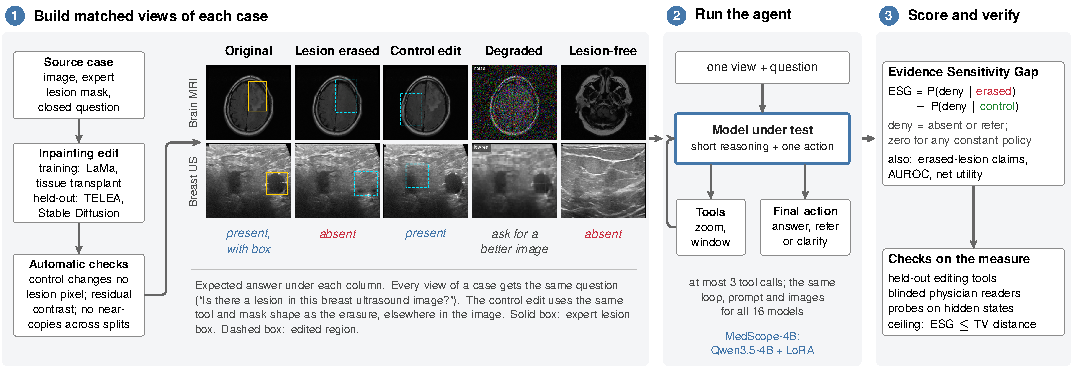
\includegraphics[width=\textwidth]{figures/fig1_framework.pdf}
\end{center}
\vspace{-0.3cm}
\caption{The Counterfactual Evidence Framework, shown with real images from the pipeline (one brain MRI case and one breast ultrasound case). (1) Each source case is edited with an inpainting tool and checked automatically, giving matched views that are all asked the same question: the original; the erasure ($E$, dilated lesion mask inpainted); a control edit of the same shape and tool elsewhere ($C_{\text{far}}$); a degraded view; and an unedited lesion-free image, with the expected answer under each. The same-site ring control ($C_{\text{ring}}$) and the restored and half-erased views of Stage~0 are not shown. (2) Every model, frontier, open or trained, runs the same agent loop with the same prompt, tools and images. (3) What is reported, and how the measurement itself is checked.}
\label{fig:framework_overview}
\vspace{-0.2cm}
\end{figure*}

\subsection{Counterfactual Views and Symmetric Controls}
\label{subsec:method_views}
We construct counterfactual episodes from public medical segmentation datasets where each case consists of an image $I$ of height $h$ and width $w$, an expert binary lesion mask $M$ (excluding lesions smaller than $20\text{ px}$ or exceeding $20\%$ of the image area), and a clinical question $Q$ whose ground-truth answer depends on the presence of the segmented lesion. To isolate visual evidence while controlling for editing artifacts and anatomical location, we construct five core view types per case:
\begin{enumerate}[leftmargin=*,nosep]
    \item \textbf{Original ($O$):} The unmodified image $I$. Expected action: correct positive answer with a bounding box localizing the lesion.
    \item \textbf{Target removal ($E$):} The lesion mask $M$ is morphologically dilated by $5\text{ px}$ ($M_{\text{dil}}$) and inpainted using LaMa \citep{suvorov2022lama}. Expected action: explicit absent answer (\emph{``No''} to \emph{``Is there\dots?''}, \emph{``Yes''} to \emph{``Is \dots\ healthy?''}, or \emph{``No abnormality''} to open queries).
    \item \textbf{Random-removal control ($C_{\text{far}}$):} The identical dilated mask shape $M_{\text{dil}}$ is translated to a random foreground tissue location that does not intersect $M_{\text{dil}}$ and is inpainted with the exact same tool. No pixel within the true lesion $M$ is altered. Expected action: the original positive answer and lesion bounding box.
    \item \textbf{Degraded view ($D$):} The image is corrupted via Gaussian blur ($\sigma = \max(h,w)/40$), additive Gaussian noise ($\sigma = 60$), $8\times$ down/up-sampling, severe JPEG compression, motion blur, or substitution with an image of a different anatomical modality. Expected action: \texttt{clarify}.
    \item \textbf{Natural negative ($N$):} An unedited lesion-free image from the same modality and source, assigned the exact same reward structure as target removal $E$. Including $N$ ensures that a shortcut policy that simply answers \emph{``absent''} whenever it detects an inpainting artifact cannot succeed on unedited healthy images.
\end{enumerate}

\textbf{Training-only views and held-out editing tools.} During training, we additionally construct \emph{lesion-insertion} views (copying a real segmented lesion into a healthy training image) and apply a second erasure mechanism---\emph{tissue transplant} (Poisson-blended healthy tissue from the same image)---to half of the training cases. To test whether evidence sensitivity transfers to unseen editing mechanisms, test-set target removals and random-removal controls are regenerated on the exact same masks using two held-out inpainting tools never seen in training: classical partial differential equation inpainting (\textbf{TELEA} \citep{telea2004image}) and \textbf{Stable Diffusion} inpainting \citep{rombach2022high}. We also evaluate a Stage-1 \emph{tool-family} training variant in which each training case's erasure and control edit are generated with one tool sampled from $\{\text{LaMa}, \text{blur fill}, \text{mean fill with noise}, \text{shuffled pixels}\}$.

\textbf{Same-site ring controls and graded evidence.} Because $C_{\text{far}}$ edits tissue away from the lesion while $E$ edits at the lesion, a model could theoretically learn a location-conditioned shortcut (\emph{``edited at the queried anatomical site means absent''}). To test this directly, we introduce three site-matched views in Stage 0 of our framework: (i) the \textbf{Same-Site Ring Control ($C_{\text{ring}}$)}, where the inpainting tool fills an area-matched ring starting $2\text{ px}$ outside the lesion boundary while leaving all lesion pixels intact; (ii) the \textbf{Restored view ($R$)}, formed by taking the erased view $E$ and restoring the lesion's original pixels; and (iii) the \textbf{Partial erasure ($P$)}, where exactly half of the lesion mask is erased with LaMa to provide graded visual evidence.

\textbf{Automated quality control.} All edited views pass through a strict, automated quality control pipeline without human intervention: (1) the erased region's contrast against a surrounding $6\text{--}14\text{ px}$ ring must be $\le \max(1.0, 0.35 \times \text{contrast}_{\text{before}})$, and a trained edit detector must score the region below $0.5$; (2) zero lesion pixels may change in $C_{\text{far}}$; (3) near-duplicate images across splits are prevented via $64$-bit difference hashing and pixel correlation across all $6,849$ unedited images; and (4) views undergo adversarial filtering until a texture classifier separates target from random edits at $\text{AUC} \le 0.60$ ($0.56$ on the main test set; a hand-crafted shortcut classifier on training views reached $\text{AUC } 0.59$).

\subsection{Evidence Sensitivity Metrics, Cost Matrix, and Abstention Ceiling}
\label{subsec:method_metrics}
Let a model or decision policy $\pi$ map a view and question $(V, Q)$ to a terminal action $a \in \{\text{claim}, \text{absent}, \text{refer}, \text{clarify}\}$. We define the primary metric, the \textbf{Evidence Sensitivity Gap (ESG)}, as the difference in denial/referral probability between target removal and the matched random-removal control:
\begin{equation}
\label{eq:esg}
\begin{split}
\text{ESG}(\pi) = {}& P\big(a \in \{\text{absent}, \text{refer}\} \mid E\big)\\
&- P\big(a \in \{\text{absent}, \text{refer}\} \mid C_{\text{far}}\big).
\end{split}
\end{equation}
By construction, $\text{ESG}(\pi) = 0$ for any constant policy (always claiming, always denying, or always referring) and, in expectation, for any policy that ignores the image or reacts identically to both edits. We also report \textbf{Strict ESG} (counting explicit $\text{absent}$ answers only) and the site-matched gap $\text{ESG}_{\text{site}} = P(a \in \{\text{absent}, \text{refer}\} \mid E) - P(a \in \{\text{absent}, \text{refer}\} \mid C_{\text{ring}})$.

Alongside ESG, we report: \textbf{Erased-lesion claims} $P(a = \text{claim} \mid E)$; \textbf{Healthy-image claims} $P(a = \text{claim} \mid N)$; \textbf{covered-and-correct rate (CCR)}, the share of answerable views ($O \cup C_{\text{far}}$) answered correctly; \textbf{Grounded accuracy}, the fraction of answerable views answered correctly with a predicted bounding box achieving $\text{IoU} \ge 0.3$ against $M$; \textbf{Area Under the Risk--Coverage Curve (AURC)} \citep{geifman2017selective} for selective prediction; and \textbf{Net Utility}, the mean reward across all views under a pre-specified clinical cost matrix (Table~\ref{tab:cost_matrix}). A correct answer on $O \cup C_{\text{far}}$ with box $\text{IoU} \ge 0.3$ earns a $+0.5$ grounding bonus (boxes covering $>50\%$ of the image earn no bonus), unparseable outputs score $-1.0$, and each tool call beyond the first incurs a $-0.05$ penalty.

\begin{table}[!t]
\caption{Pre-specified clinical cost matrix: reward per view ($O$ original, $C_{\text{far}}$ control edit, $E$ erasure, $N$ lesion-free, $D$ degraded). A $+0.5$ grounding bonus is added on Original and Random-removal views when the predicted bounding box achieves $\text{IoU} \ge 0.3$ (with area $\le 50\%$ of the image).}
\label{tab:cost_matrix}
\begin{center}
\footnotesize
\begin{tabular}{lcccc}
\toprule
\textbf{View} & \textbf{Correct} & \textbf{False claim / wrong} & \textbf{Refer} & \textbf{Clarify} \\
\midrule
$O$, $C_{\text{far}}$ & $+1.0$ & $-2.0$ ($-4.0$ critical) & $-0.3$ & $-0.3$ \\
$E$, $N$ & $+1.0$ & $-2.0$ & $+0.5$ & $-0.5$ \\
$D$ & $+0.25$ & $-2.0$ & $0.0$ & $+0.5$ \\
\bottomrule
\end{tabular}
\end{center}
\end{table}

\textbf{Separating discrimination from threshold and the Abstention Ceiling.} Because ESG and Net Utility evaluate discrete decisions at a fixed operating point, we separately compute threshold-free non-parametric discrimination---$\text{AUROC}_{\text{far}}$ ($E$ vs.\ $C_{\text{far}}$) and $\text{AUROC}_{\text{site}}$ ($E$ vs.\ $C_{\text{ring}}$)---alongside raw denial rates and within-case single-turn decision log-odds shifts $\Delta s(V) = s(V) - s(O)$, where $s(x) = \log p(\text{present reply} \mid x) - \log p(\text{absent reply} \mid x)$ evaluated on identical reply tokens within each case. Furthermore, we formalize why post-hoc abstention or test-time evidence combiners cannot create evidence sensitivity beyond their inputs:

\textbf{Proposition 1 (Abstention Ceiling).} \emph{Let $S = f(V, Q)$ be any set of signals extracted from view $V$ and question $Q$ (e.g., model logits, confidence scores, or multi-agent outputs), and let $\pi: S \to \{\text{claim}, \text{absent}, \text{refer}, \text{clarify}\}$ be any deterministic or randomized decision policy operating solely on $S$. Let $D = \mathbb{I}[\pi(S) \in \{\text{absent}, \text{refer}\}]$. Then}
\begin{equation}
\label{eq:abstention_ceiling}
\begin{split}
\text{ESG}(\pi) &= P(D = 1 \mid E) - P(D = 1 \mid C_{\text{far}})\\
&\le \text{TV}\big(P(S \mid E),\, P(S \mid C_{\text{far}})\big),
\end{split}
\end{equation}
\emph{where $\text{TV}(P, Q) = \sup_{A} |P(A) - Q(A)|$ is the total-variation distance.}

\emph{Proof.} For the binary random variable $D = g(S)$, $|P(D=1 \mid E) - P(D=1 \mid C_{\text{far}})| = \text{TV}(P(D \mid E), P(D \mid C_{\text{far}}))$. By the data-processing inequality for $f$-divergences (and specifically total variation) applied to the Markov chain $V \to S \to D$, $\text{TV}(P(D \mid E), P(D \mid C_{\text{far}})) \le \text{TV}(P(S \mid E), P(S \mid C_{\text{far}}))$. $\square$

Consequently, post-hoc abstention rules on existing signals $S$ cannot raise ESG above the separation already encoded in $S$, even though they can substantially raise Net Utility by routing uncertain cases to the $+0.5$ referral reward on $E$ and $N$.

\subsection{Reference Agent (\texttt{MedScope-4B}) and Pre-Registered Methods Tested}
\label{subsec:method_agent}
\textbf{Agent protocol and architecture.} In every episode, the model receives the image (PNG, long side $\le 768\text{ px}$) and question under an identical multi-turn protocol allowing at most $3$ tool calls. At each turn, the model emits brief reasoning followed by one tagged JSON action: \texttt{zoom} (integer bounding box $[x_1, y_1, x_2, y_2] \in [0, 1000]^4$ on the original image, returning a cropped view), \texttt{window} (intensity center and width in $[0, 255]$, returning a contrast-adjusted view), \texttt{answer} (final text answer, optional evidence bounding box, and confidence), \texttt{refer} (image is usable but finding is indeterminate), or \texttt{clarify} (image is degraded/unusable or depicts the wrong anatomy).

Our reference agent, \texttt{MedScope-4B}, is built on \texttt{Qwen3.5-4B} with a frozen vision encoder and LoRA adapters ($\text{rank } 16$, $\alpha = 32$, dropout $0.05$) applied to all linear layers of the language model. Training trajectories are synthesized automatically from dataset labels alone: trajectories invoke \texttt{zoom} on a jittered box around the lesion (mandatory when the lesion covers $<2\%$ of the image), invoke \texttt{window} on $30\%$ of greyscale images, and emit the expected terminal action with concise template reasoning. Half of the training questions are rephrased using four training paraphrases, while three distinct paraphrases are held out for testing. \texttt{MedScope-4B} is trained in three stages:
\begin{itemize}[leftmargin=*,nosep]
    \item \textbf{Stage 1 (Counterfactual SFT):} Supervised fine-tuning on $16,000$ counterfactual and control views for one epoch ($3,706$ optimizer steps) at learning rate $2\times 10^{-4}$.
    \item \textbf{Stage 2 (Rejection-Sampling Fine-Tuning):} Sampling $k=4$ rollouts per view at temperature $T=1.2$, retaining the highest-reward successful trajectory (repeating hard views $\times 3$), and fine-tuning at learning rate $5\times 10^{-5}$.
    \item \textbf{Stage 3 (General-VQA Replay):} Fine-tuning on $5,000$ views mixing MedScope counterfactual trajectories with standard training-split questions from VQA-RAD \citep{lau2018vqarad}, SLAKE \citep{liu2021slake}, and PathVQA \citep{he2020pathvqa} at learning rate $5\times 10^{-5}$.
\end{itemize}
Under our pre-registered selection rule (committed 1 November 2026 before any v4 data or model existed), Stage 3 is selected over Stage 2 if validation net utility satisfies $U_3 \ge U_2 - 0.02$ and healthy-image claims satisfy $H_3 \le H_2 + 0.02$. On the $540$-case validation set ($1,473$ views), $(U, H)$ progressed from $(0.585, 13.6\%)$ in Stage 1 to $(0.610, 12.7\%)$ in Stage 2 and $(0.613, 7.7\%)$ in Stage 3; Stage 3 was thus locked as \texttt{MedScope-4B} and evaluated once on all test sets without post-hoc tuning.

\textbf{Pre-registered competing methods, multi-agent verifiers, and probes.} To test whether popular post-training alignment or test-time verification techniques improve evidence discrimination beyond Stage-1 counterfactual SFT, we evaluate twelve pre-registered training or system arms against matched controls:
(1) \textbf{Check C1}: matched vs.\ unmatched control edit geometry and tool;
(2) \textbf{Checks C2 \& C3}: removal-based DPO \citep{rafailov2023dpo} applied either after standard non-counterfactual SFT or on top of the counterfactual recipe;
(3) \textbf{Check C4 (Control-Matched Counterfactual Consistency, CMCC)}: a paired-view consistency objective optimizing
\begin{equation}
\label{eq:cmcc}
\begin{split}
\mathcal{L}_{\text{CMCC}} = {}& \mathcal{L}_{\text{traj}} + 0.5 \cdot \text{softplus}\big(2 - (s(C_{\text{far}}) - s(E))\big)\\
&+ 0.5 \cdot \big(s(O) - s(C_{\text{far}})\big)^2 + 0.5 \cdot \mathcal{L}_{\text{first-action}},
\end{split}
\end{equation}
tested across three seed pairs against a matched-compute replay-only control;
(4) higher adapter capacity (\textbf{LoRA rank 64}) and \textbf{Vision Encoder LoRA} at learning rates $2\times 10^{-4}$ and $2\times 10^{-5}$;
(5) \textbf{GRPO} \citep{shao2024deepseekmath} trained directly on the cost-matrix reward for $150$ steps;
(6) \textbf{Counterfactual Multi-Agent Readers (v10 and v11)} combining a direct reader, a question-blind reader, a dedicated lesion segmenter, an erase-and-re-ask counterfactual verifier, and a trained arbiter (trained in-sample in v10 and on out-of-sample reports in v11);
(7) a split-validation screening funnel of \textbf{270 decision policies} (128 Stage-A policies over stored agent/multi-agent outputs and 142 Stage-B policies incorporating test-time image augmentations, crops, token probabilities, \texttt{Qwen2.5-VL-7B}, and segmenter scores); and
(8) \textbf{Stage-1 Tool-Family training} with and without CMCC.
Finally, we conduct a \textbf{blinded two-physician reader study} ($128$ main-test views across $O, E, C_{\text{far}}, N$) and train $5$-fold case-grouped \textbf{logistic regression linear probes} \citep{alain2016understanding} on hidden states (last prompt token and mean image tokens across $8$ layers) to compare internal feature separation against behavioral output AUROC.

\textbf{Design choices.} Table~\ref{tab:design} gives the reason for each fixed choice and where its effect is checked.


%%%%%%%%% METHOD %%%%%%%%%

\section{Experiments}
\label{sec:experiments}
%%%%%%%%% EXPERIMENTS %%%%%%%%%

\subsection{Datasets, Baselines, and Statistical Protocol}
\label{subsec:exp_setup}
\textbf{Datasets.} We chose sources that release expert lesion masks (needed to erase a lesion and to place a control edit of the same shape) and lesion-free images of the same imaging type, covering five imaging types with different kinds of findings (focal mucosal, mass, opacity, tumour). Training, validation, and internal main-test splits are constructed from five public sources: SLAKE \citep{liu2021slake} (CT and MRI of several body regions), Kvasir-SEG \citep{jha2020kvasir} supplemented with HyperKvasir \citep{borgli2020hyperkvasir} normal landmarks (colonoscopy), ChestX-Det \citep{liu2020chestxdet} from NIH ChestX-ray14 (chest X-ray), BUSI \citep{al2020dataset} (breast ultrasound), and TCGA-LGG \citep{buda2019association} (brain MRI FLAIR). After quality checks, training comprises $1,508$ SLAKE and colonoscopy cases plus $1,792$ chest X-ray, breast ultrasound, and brain MRI cases, alongside $690$ unedited lesion-free images. Validation contains $540$ cases ($1,473$ views). The internal \textbf{main test set} contains $507$ cases ($219$ with expert lesion masks and $288$ lesion-free natural negatives), yielding $1,115$ total views ($219$ original, $219$ target removal, $219$ random removal, $170$ degraded, and $288$ natural negatives), split strictly by patient ID (ChestX-Det, TCGA-LGG) or near-copy perceptual groups (SLAKE, Kvasir-SEG, BUSI).

To evaluate out-of-distribution generalization and prevent overfitting, we test on six additional cohorts (summarized in Table~\ref{tab:datasets_overview}): \textbf{External centres} ($169$ cases from CVC-ClinicDB, QaTa-COV19, BUS-BRA, and BraTS-Africa 2023), \textbf{Fresh internal} ($76$ unused ChestX-Det patients), \textbf{Fresh external} ($316$ cases from BraTS 2023 meningioma, BUS-UCLM, SIIM-ACR pneumothorax, and ETIS-LaribPolypDB), \textbf{Held-out wordings} ($373$ main-test cases with three unseen question paraphrases), \textbf{Standard VQA} ($1,051$ test items from VQA-RAD \citep{lau2018vqarad}, SLAKE English \citep{liu2021slake}, and PathVQA \citep{he2020pathvqa}), and \textbf{Held-out editing tools} ($125$ and $219$ main-test cases remade with unseen TELEA \citep{telea2004image} and Stable Diffusion \citep{rombach2022high} inpainting). A $64$-bit difference-hash audit across all $6,849$ unedited images confirmed that exactly one image recurred across splits (a lesion-free ChestX-Det validation image matching one SIIM fresh-external case; excluding it alters fresh-external ESG by $+0.002$, CCR by $+0.003$, and net utility by $+0.007$).

\textbf{Data leakage and patient-level splits.} Every image is assigned to its split before any view is built, so all views of an image stay in its split, and every fitted quantity (the stage-3 selection rule, the 270 decision policies, the probes and the review checks) uses training or validation data only. Splits are per patient where the source releases patient identifiers (ChestX-Det via NIH ChestX-ray14, TCGA-LGG) and otherwise per group of near-identical images (SLAKE, Kvasir-SEG with HyperKvasir, BUSI); for the latter, two images of one patient that are not near-copies can fall into different splits, and we cannot rule this out. A cross-set audit hashed every unedited image of every split and cohort: no case, patient or group identifier is shared by any two sets, and exactly one image recurs (a ChestX-Det validation image). Resampling whole patients or groups instead of cases widens the intervals by at most $0.01$ (main test) and $0.03$ (fresh external); all $27$ primary comparisons stay significant, and one secondary comparison crosses $0.05$ (fresh-external ESG vs.\ \texttt{Claude Opus 5.5}, $p = 0.037 \to 0.060$).

\begin{table*}[!t]
\caption{Summary of the internal main test set (top) and the six external, confirmatory, and stress-test evaluation cohorts (bottom). $^{\dagger}$Lesion-free images built for the fresh external set; $316$ cases were evaluated in total.}
\label{tab:datasets_overview}
\vspace{-0.2cm}
\begin{center}
\small
\begin{adjustbox}{max width=\linewidth}
\begin{tabular}{llccc}
\toprule
\textbf{Cohort / Source} & \textbf{Imaging Modality or Composition} & \textbf{Masked} & \textbf{Lesion-Free} & \textbf{Total Cases (Views)} \\
\midrule
SLAKE & CT / MRI (near-copy split) & 17 & 90 & 107 \\
Kvasir-SEG + HyperKvasir & Colonoscopy (near-copy split) & 83 & 91 & 174 \\
ChestX-Det & Chest X-ray (patient split) & 41 & 50 & 91 \\
BUSI & Breast ultrasound (near-copy split) & 42 & 15 & 57 \\
TCGA-LGG & Brain MRI FLAIR (patient split) & 36 & 42 & 78 \\
\textbf{Main Test Total} & \textbf{5 modalities (170 degraded views)} & \textbf{219} & \textbf{288} & \textbf{507 (1,115)} \\
\midrule
External centres & CVC-ClinicDB (40), QaTa-COV19 (20), & 119 & 50 & 169 \\
 & BUS-BRA (45), BraTS-Africa 2023 (64) & & & \\
Fresh internal & Unused ChestX-Det test patients & 36 & 40 & 76 \\
Fresh external & BraTS meningioma (82), BUS-UCLM (99), & 168 & 150$^{\dagger}$ & 316 \\
 & SIIM pneumothorax (96), ETIS-Larib (39) & & & \\
Held-out wordings & Main test with 3 test-only paraphrases & -- & -- & 373 \\
Standard VQA & VQA-RAD (451), SLAKE (300), PathVQA (300) & -- & -- & 1,051 \\
Held-out editing tools & TELEA, Stable Diffusion, Transplant & 125 / 219 & -- & 125 / 219 \\
\bottomrule
\end{tabular}
\end{adjustbox}
\end{center}
\vspace{-0.2cm}
\end{table*}

\textbf{Baselines and statistical protocol.} We compare \texttt{MedScope-4B} against nine frontier VLMs evaluated via their public APIs under provider default settings on 31 October 2026 (OpenAI \texttt{gpt-6-sol}, \texttt{gpt-6-astra}, \texttt{gpt-6.1-sol}; Anthropic \texttt{Claude Fable 5.1}, \texttt{Claude Opus 5.5}, \texttt{Claude Sonnet 5.5}; and Google \texttt{gemini-4-argon}, \texttt{gemini-3.1-pro-preview}, and \texttt{gemini-3.8-flash}), six open-weight VLMs run locally in \texttt{bfloat16} with greedy decoding (\texttt{Qwen3.5-4B} base, \texttt{MedGemma 1.5 4B}, \texttt{Lingshu-7B}, \texttt{HuatuoGPT-Vision-7B}, \texttt{Qwen2.5-VL-7B}, and \texttt{Qwen3-VL-8B}), and three trivial constant policies (stored per-view transcripts and scored outputs are in the public repository). All $95\%$ confidence intervals are computed via $2,000$ case-clustered bootstrap resamples (resampling all views of a case together; resampling whole patients or near-copy groups widens intervals by $\le 0.01$ on the main test and $\le 0.03$ on fresh external). Two-tailed paired bootstrap $p$-values across the $27$ primary comparisons (ESG, erased-lesion claims, and net utility against the nine frontier models) are evaluated against a Bonferroni-corrected threshold of $\alpha = 0.05/27$. Each training stage used one NVIDIA A100 40 GB GPU for about $4\text{ h}$ (later pilots used an A100 80 GB and an RTX PRO 6000 96 GB) (PyTorch 2.11, Transformers 5.22.1, PEFT 0.21.2); frontier API runs on the main test cost US\$132, and all 48 API runs cost US\$373 total.

\subsection{Main Benchmark Results and Frontier Model Robustness}
\label{subsec:exp_main}
Table~\ref{tab:main_results} and Figure~\ref{fig:frontier_vs_medscope_main}a present the main benchmark results across all $507$ cases ($1,115$ views). While all nine frontier VLMs achieve high answerable accuracy ($\text{CCR } 0.829\text{--}0.888$), they claim the queried lesion on $41.1\%$ (\texttt{gemini-4-argon}) to $61.6\%$ (\texttt{gemini-3.8-flash}) of target-erased views, with ESG between $0.269$ and $0.470$. In contrast, \texttt{MedScope-4B} achieves an ESG of $0.758$ $[0.701, 0.815]$, reduces erased-lesion claims to $9.6\%$ $[6.1, 13.7]$ and healthy-image claims to $7.6\%$ $[4.8, 10.9]$, maintains a competitive CCR of $0.849$, and reaches a Net Utility of $0.732$ $[0.649, 0.813]$. Furthermore, \texttt{MedScope-4B} correctly asks to \texttt{clarify} on all $170/170$ degraded views.

\begin{table*}[!t]
\caption{Main test performance across $507$ cases ($1,115$ views) under the identical multi-turn agent protocol. Erased \% denotes false finding claims on $219$ target-erased views; Healthy \% denotes false claims on $288$ unedited lesion-free views; CCR is measured over $438$ answerable views ($O \cup C_{\text{far}}$). Bracketed ranges for \texttt{MedScope-4B} indicate $95\%$ case-clustered bootstrap confidence intervals.}
\label{tab:main_results}
\vspace{-0.2cm}
\begin{center}
\small
\begin{adjustbox}{max width=\linewidth}
\begin{tabular}{lccccc}
\toprule
\textbf{Model} & \textbf{CCR} $\uparrow$ & \textbf{ESG} $\uparrow$ & \textbf{Erased \%} $\downarrow$ & \textbf{Healthy \%} $\downarrow$ & \textbf{Net Utility} $\uparrow$ \\
\midrule
\textbf{MedScope-4B (Ours)} & 0.849 & \textbf{0.758} [0.701, 0.815] & \textbf{9.6} [6.1, 13.7] & \textbf{7.6} [4.8, 10.9] & \textbf{0.732} [0.649, 0.813] \\
\midrule
gemini-4-argon & 0.874 & 0.470 & 41.1 & 9.0 & 0.565 \\
Claude Sonnet 5.5 & 0.870 & 0.402 & 48.4 & 16.7 & 0.381 \\
gemini-3.1-pro-preview & 0.849 & 0.384 & 51.6 & 26.7 & 0.306 \\
gpt-6-sol & 0.829 & 0.342 & 51.6 & 25.7 & 0.261 \\
Claude Fable 5.1 & 0.856 & 0.342 & 52.1 & 23.3 & 0.255 \\
Claude Opus 5.5 & 0.863 & 0.329 & 53.9 & 23.6 & 0.358 \\
gpt-6.1-sol & \textbf{0.888} & 0.324 & 58.9 & 30.9 & 0.276 \\
gpt-6-astra & 0.886 & 0.306 & 58.9 & 27.8 & 0.309 \\
gemini-3.8-flash & 0.868 & 0.269 & 61.6 & 27.8 & 0.263 \\
\midrule
Lingshu-7B & 0.527 & 0.416 & 32.0 & 12.5 & $-0.249$ \\
Qwen3.5-4B (base) & 0.758 & 0.338 & 42.0 & 19.4 & 0.134 \\
Qwen3-VL-8B & 0.553 & 0.297 & 12.8 & 12.5 & 0.186 \\
MedGemma 1.5 4B & 0.674 & 0.283 & 54.3 & 24.0 & $-0.255$ \\
HuatuoGPT-Vision-7B & 0.498 & 0.265 & 30.1 & 22.9 & $-0.426$ \\
Qwen2.5-VL-7B & 0.144 & 0.146 & 5.5 & 24.7 & $-0.742$ \\
\midrule
Always claims finding & 1.000 & 0.000 & 100.0 & 100.0 & $-0.478$ \\
Always says absent & 0.000 & 0.000 & 0.0 & 0.0 & $-0.848$ \\
Always refers & 0.000 & 0.000 & 0.0 & 0.0 & 0.110 \\
\bottomrule
\end{tabular}
\end{adjustbox}
\end{center}
\vspace{-0.2cm}
\end{table*}

\begin{figure*}[!t]
\begin{center}
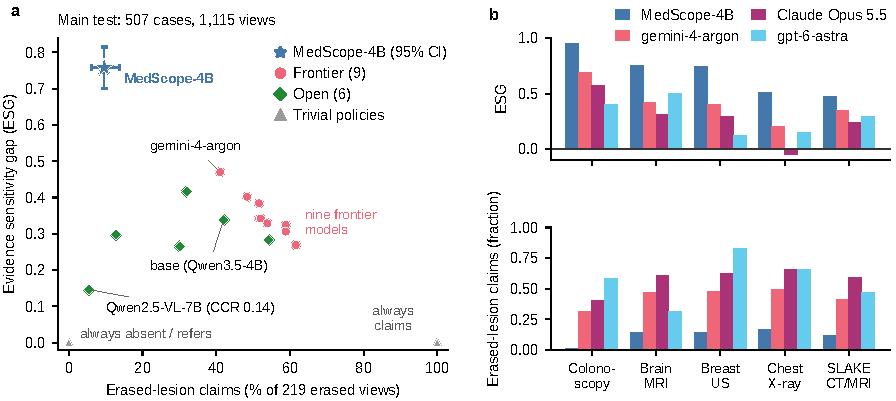
\includegraphics[width=\textwidth]{figures/fig2_main_test.pdf}
\end{center}
\vspace{-0.3cm}
\caption{Frontier VLMs claim $41$--$62\%$ of erased findings; \texttt{MedScope-4B} claims $9.6\%$, on every imaging type. Main test ($507$ cases, $1{,}115$ views). (a) ESG against the share of the $219$ erased views on which each model claims the finding: \texttt{MedScope-4B} (bars: $95\%$ bootstrap intervals), the nine frontier VLMs, the six open VLMs and the trivial policies (ESG $0$). Lower claims alone are not better: \texttt{Qwen2.5-VL-7B} claims least among the open models ($5.5\%$) but answers almost nothing correctly (CCR $0.144$, ESG $0.146$). (b) By imaging type, \texttt{MedScope-4B} against the three flagships: ESG (top) and erased-lesion claims as a fraction (bottom); values in Supplementary Table~\ref{tab:modality_breakdown}.}
\label{fig:frontier_vs_medscope_main}
\vspace{-0.2cm}
\end{figure*}

In paired bootstrap comparisons against each of the nine frontier models, \texttt{MedScope-4B} improves ESG by $+0.288$ to $+0.489$ (vs.\ \texttt{gemini-4-argon}: $+0.288$ $[0.208, 0.367]$, all $p < 0.001$), lowers erased-lesion claims by $-0.315$ to $-0.521$ (all $p < 0.001$), and increases Net Utility by $+0.168$ to $+0.477$ (all $p \le 0.001$), surviving Bonferroni correction across all $27$ primary tests. CCR differences between \texttt{MedScope-4B} and the frontier models range from $-0.039$ to $+0.021$ ($p \ge 0.12$; confidence intervals reach $-0.09$, so formal equivalence is not established), and healthy-image claims are significantly lower than eight of nine frontier models ($p \le 0.001$; vs.\ \texttt{gemini-4-argon} $-0.014$, $p = 0.59$). Relative to its untrained \texttt{Qwen3.5-4B} base model, \texttt{MedScope-4B} improves ESG by $+0.420$ $[0.338, 0.498]$ (and by $+0.475$ over untrained \texttt{MedGemma 1.5 4B}). Table~\ref{tab:main_results} illustrates why erased-lesion claims cannot be evaluated without matched controls: ranking models by erased claims alone produces a \textbf{ranking reversal} that prefers \texttt{Qwen2.5-VL-7B} ($5.5\%$ erased claims) over \texttt{MedScope-4B} ($9.6\%$), even though \texttt{Qwen2.5-VL-7B} achieves this solely by defaulting to \emph{``absent''} on nearly all inputs ($\text{CCR } 0.144$, $\text{ESG } 0.146$, Net Utility $-0.742$).

As shown in Figure~\ref{fig:frontier_vs_medscope_main}b (and Supplementary Table~\ref{tab:modality_breakdown}), \texttt{MedScope-4B} outperforms the frontier flagships across all five imaging modalities, achieving an ESG / erased-claim fraction / net utility of $0.95 / 0.01 / 1.06$ on Colonoscopy (vs.\ $0.40\text{--}0.69$ ESG and $0.31\text{--}0.58$ erased claims for flagships), $0.75 / 0.14 / 0.75$ on Brain MRI, $0.74 / 0.14 / 0.78$ on Breast Ultrasound, $0.51 / 0.17 / 0.40$ on Chest X-ray (where \texttt{Claude Opus 5.5} drops to $-0.05$ ESG), and $0.47 / 0.12 / 0.22$ on SLAKE CT/MRI.

\textbf{Prompting, reasoning, tool-use, and lesion-size robustness.} To test whether frontier false claims stem from prompt phrasing or sub-optimal inference settings, we re-evaluated \texttt{gemini-4-argon}, \texttt{Claude Opus 5.5}, and \texttt{gpt-6-astra} on a $150$-case subset across six regimes: Default, Cautious prompt, Solved in-context examples, Highest reasoning budget, Highest image resolution setting, and a Plain free-text prompt without tools (Figure~\ref{fig:readers_robustness}b1 and Supplementary Table~\ref{tab:robustness_prompts}). Across all six conditions, frontier models continue to claim $36.8\%$ to $66.2\%$ of erased lesions ($\text{ESG } 0.250\text{--}0.500$), whereas \texttt{MedScope-4B} achieves $0.750$ ESG and $7.4\%$ erased claims ($p \le 0.001$ on ESG and $p \le 0.034$ on utility in every condition). Furthermore, \texttt{MedScope-4B} is unchanged on held-out question wordings ($373$ cases; net utility change $+0.006$ $[-0.033, 0.041]$) and ranks first under all five alternative clinical cost matrices tested. Refusing tool calls (\texttt{zoom} and \texttt{window}) at test time leaves \texttt{MedScope-4B} ESG unchanged ($0.753$ vs.\ $0.758$, $p = 0.92$) while reducing net utility by $0.092$ ($p = 0.003$) and CCR by $0.053$: the tools add accuracy on real lesions rather than evidence sensitivity. Stratified by lesion-area quartiles (Figure~\ref{fig:readers_robustness}b2), \texttt{MedScope-4B} ESG scales monotonically from $0.545$ in Q1 ($18.2\%$ erased claims on the smallest lesions) to $0.741$ (Q2), $0.836$ (Q3), and $0.909$ in Q4 ($1.8\%$ erased claims), whereas the three flagships stay within ESG $0.20\text{--}0.56$ in every quartile.

\subsection{Active Ingredients of Counterfactual Training and Held-Out Editing Tools}
\label{subsec:exp_ablations_tools}
To isolate what drives \texttt{MedScope-4B}'s evidence sensitivity, we conduct Stage-1 training ablations (Figure~\ref{fig:heldout_tools_and_ablations}c and Supplementary Table~\ref{tab:ablations_and_factorial}A), a $2\times 2$ factorial decomposition of training views (Figure~\ref{fig:heldout_tools_and_ablations}b and Supplementary Table~\ref{tab:ablations_and_factorial}B), and transfer evaluations on unseen inpainting tools (Figure~\ref{fig:heldout_tools_and_ablations}a and Supplementary Table~\ref{tab:heldout_tools}).

\begin{figure*}[!t]
\begin{center}
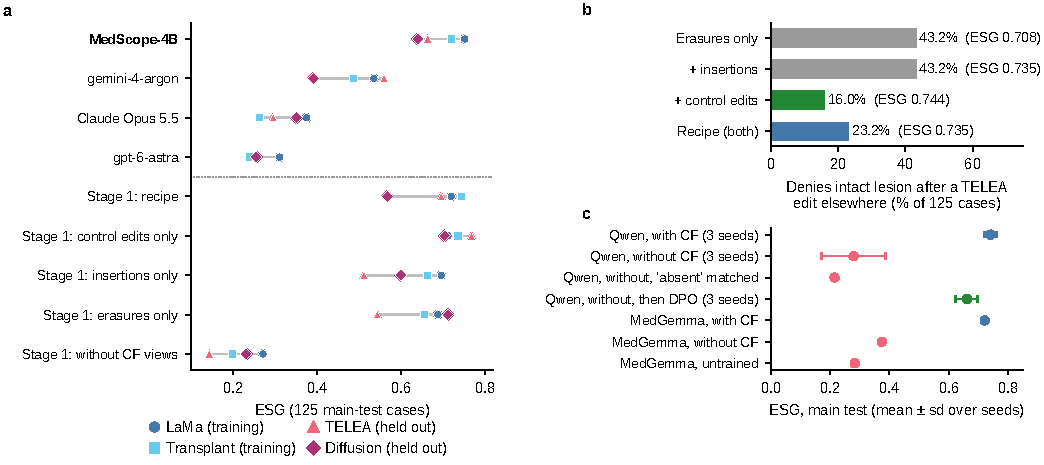
\includegraphics[width=\textwidth]{figures/fig3_tools_ablations.pdf}
\end{center}
\vspace{-0.3cm}
\caption{\texttt{MedScope-4B} leads every flagship on every editing tool, and the control edit, not lesion insertion, removes the ``edited means absent'' shortcut. (a) ESG on $125$ main-test cases whose erasures and control edits were remade with each tool on the same masks: two training tools (LaMa, tissue transplant) and two held-out tools (TELEA, Stable Diffusion). (b) $2\times 2$ factorial of training-only components (Stage~1, seed~0): share of $125$ intact lesions denied after a TELEA edit elsewhere in the image, with main-test ESG in brackets; control edits, not lesion insertions, remove the ``edited means absent'' shortcut. (c) Main-test ESG of Stage-1 arms (mean $\pm$ sd over three seeds where marked): blue, with counterfactual (CF) views; vermilion, without; green, without CF views followed by removal-based DPO (check C2); the MedGemma rows replicate the recipe on a second architecture.}
\label{fig:heldout_tools_and_ablations}
\vspace{-0.2cm}
\end{figure*}

\textbf{Counterfactual views vs.\ label priors.} Removing counterfactual views from Stage-1 SFT causes ESG to collapse from $0.741 \pm 0.019$ to $0.279 \pm 0.107$ across three seeds (per-seed differences $+0.525, +0.539, +0.324$, all $p < 0.001$; external centres ESG $0.622 \pm 0.030$ vs.\ $0.389 \pm 0.043$) and increases erased-lesion claims from $13.2\%$ to $67.6\%$ (Supplementary Table~\ref{tab:ablations_and_factorial}A). To verify that this gain is not merely an artifact of exposing the model to more negative (\emph{``absent''}) labels during training, we trained an arm without counterfactual views but matched the exact proportion of \emph{``absent''} answers using natural lesion-free images; this arm achieved only $0.215$ ESG ($73.5\%$ erased claims; paired difference $+0.521$ $[0.440, 0.600]$). Replicating the Stage-1 recipe on a medical-specialized architecture, \texttt{MedGemma 1.5 4B}, similarly boosts ESG from $0.283$ (untrained) and $0.374$ (SFT without counterfactuals) to $0.721$ ($+0.347$ $[0.276, 0.425]$). Stages 2 and 3 provide modest polishing over Stage 1 on the main test (net utility $+0.040$, $p = 0.15$; ESG $+0.023$, $p = 0.39$) while halving healthy-image claims on validation ($13.6\% \to 7.7\%$).

\textbf{How control edits suppress the ``edited means absent'' shortcut.} In the $2\times 2$ factorial ablation (Figure~\ref{fig:heldout_tools_and_ablations}b and Supplementary Table~\ref{tab:ablations_and_factorial}B), training on target erasures alone achieves strong main-test ESG ($0.708$) and low erased claims ($6.8\%$). However, when evaluated on $125$ cases where an unseen tool (TELEA) performs a control edit elsewhere on the image while leaving the lesion intact, the erasures-only model falsely denies $43.2\%$ of intact lesions---having learned the shortcut that \emph{any inpainted image has no lesion}. Including random-location control edits during training cuts this false denial rate by more than half, to $16.0\%$ (control edits only) and $23.2\%$ (full recipe).

\textbf{Transfer to held-out editing tools and edit visibility.} Across the $125$-case multi-tool benchmark (Figure~\ref{fig:heldout_tools_and_ablations}a and Supplementary Table~\ref{tab:heldout_tools}A), \texttt{MedScope-4B} keeps its evidence sensitivity on both seen tools (LaMa $0.752$, Transplant $0.720$) and unseen held-out tools (TELEA $0.664$, Stable Diffusion $0.640$), outperforming every frontier flagship on every tool ($\Delta\text{ESG } +0.10$ to $+0.48$, all $p \le 0.049$). \texttt{gemini-4-argon}'s erased claims drop from $32.8\%$ on LaMa to $8.8\%$ on TELEA because it detects TELEA's smooth PDE fills as editing artifacts. Auditing edit visibility directly, a supervised ResNet-18 separates $C_{\text{far}}$ from $O$ at $\text{AUC } 0.83$ $[0.80, 0.87]$, and a linear probe on the frozen vision encoder's pooled features separates them at $\text{AUC } 0.60$ $[0.58, 0.63]$ (while separating $E$ from $C_{\text{far}}$ at $0.86$ $[0.83, 0.89]$). Zero-shot, however, \texttt{gemini-4-argon} and \texttt{gpt-6.1-sol} separate $C_{\text{far}}$ from $O$ near chance ($\text{AUC } 0.52\text{--}0.55$, while separating $E$ from $O$ at $0.70\text{--}0.75$). On the $61/219$ erasures that \texttt{gemini-4-argon} explicitly rates as unedited, \texttt{MedScope-4B} claims the lesion in only $15\%$ of cases ($8\%$ on visibly edited ones) compared to $41\%\text{--}64\%$ for the nine frontier models.

Examining where held-out ESG is lost across all $219$ cases for the Stage-1 recipe (Supplementary Table~\ref{tab:heldout_tools}B) reveals distinct failure modes by generator: on LaMa, false control denial when the unedited lesion was found is only $2.7\%$ ($5/186$), so the remaining ESG gap comes from \emph{perception} ($33/219$ real lesions missed on $O$); on TELEA, loss is driven by \emph{edit-induced denial} of intact lesions ($12.9\%$, $24/186$, including $13$ breast ultrasound cases); and on Stable Diffusion, $41/45$ false claims on $E$ point their bounding boxes at the erased site. Diffusion erasures were not reader-checked, so these sites may hold residual or regenerated lesion-like tissue; we cannot tell which.

\subsection{Pre-Registered Negative Map: Threshold Shifts vs.\ Discrimination}
\label{subsec:exp_negative_map}
A central question of our study is whether post-training alignment, consistency losses, multi-agent verification, or test-time decision policies can push evidence discrimination beyond counterfactual SFT. Figure~\ref{fig:threshold_vs_discrimination_map} and Supplementary Table~\ref{tab:negative_map_summary} synthesize our pre-registered checks (C1--C4), post-preprint training pilots, tool-family training, and the 270-policy screening funnel (numeric breakdowns in Supplementary Tables~\ref{tab:negative_map_summary}, \ref{tab:app_c1_c3}, \ref{tab:app_c4_cmcc}, and \ref{tab:app_tool_family}).

\begin{figure*}[!t]
\begin{center}
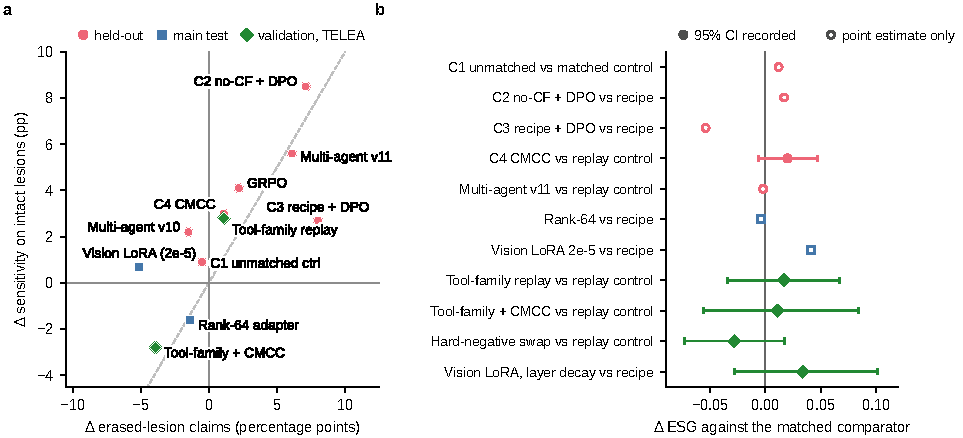
\includegraphics[width=\textwidth]{figures/fig4_negative_map.pdf}
\end{center}
\vspace{-0.3cm}
\caption{No arm shows a reliable gain over its comparator in separating erased from intact lesions: the operating point moves. (a) Each trained or system arm against its matched comparator: change in erased-lesion claims (x) and in sensitivity on intact lesions (y), in percentage points. Arms that claim more also find more, so the points follow the diagonal: the operating point moves. Held-out tools are TELEA and Stable Diffusion pooled ($219$ cases); tool-family arms are on validation TELEA views; rank-64 and vision-LoRA arms on the main test. C4 CMCC and tool-family replay nearly coincide. (b) Change in ESG for every arm with a recorded ESG difference (filled: $95\%$ interval recorded; open: point estimate only). Every recorded interval includes zero, and the point estimates lie between $-0.054$ and $+0.041$. GRPO and multi-agent v10 have no recorded ESG difference on these sets and appear only in A. The last two rows of B are the checks added after the review (Section~\ref{subsec:exp_review}). Values in Supplementary Tables~\ref{tab:negative_map_summary}--\ref{tab:app_tool_family}.}
\label{fig:threshold_vs_discrimination_map}
\vspace{-0.2cm}
\end{figure*}

\begin{figure*}[!t]
\begin{center}
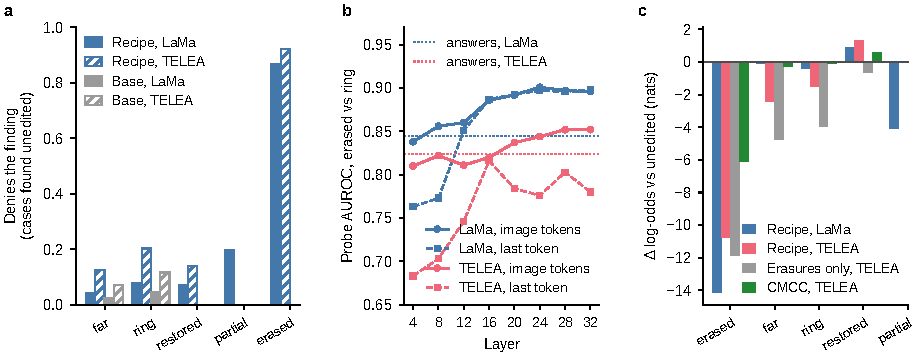
\includegraphics[width=\textwidth]{figures/fig5_stage0_probes.pdf}
\end{center}
\vspace{-0.3cm}
\caption{Denials follow the evidence rather than the edit's site, and the hidden states separate erased from intact lesions about as well as the answers do. Stage~0 on validation data (Stage-1 recipe, seed~0; untrained base model). (a) Share of intact lesions denied after each view, among cases whose unedited image the model answers present ($143$ recipe, $127$ base); the erased view is shown for reference. Partial erasure was built with LaMa only, and the restored and partial views for the recipe only. (b) Cross-validated AUROC of linear probes on the recipe's hidden states (erased vs.\ ring control) by layer, for the mean of the image tokens and the last prompt token; dotted lines give the AUROC of the recipe's own answers. (c) Within-case change of the single-turn log-odds relative to the unedited view (nats); this score failed its validity check as a cross-case score (Section~\ref{sec:discussion}) but is valid within a case.}
\label{fig:stage0_probes}
\vspace{-0.2cm}
\end{figure*}

Across all twelve trained or system arms (Supplementary Table~\ref{tab:negative_map_summary}), every modification moved the operating point---claims on erased lesions and sensitivity on intact lesions rose or fell together (Figure~\ref{fig:threshold_vs_discrimination_map}a)---without separating erased from intact lesions better than its matched comparator (Figure~\ref{fig:threshold_vs_discrimination_map}b):
\begin{itemize}[leftmargin=*,nosep]
    \item \textbf{DPO and Consistency Losses (C2--C4):} Applying removal-based DPO after non-counterfactual SFT (C2) yields no ESG improvement over our recipe on fresh external data ($0.355 \pm 0.015$ vs.\ $0.381 \pm 0.018$; single-seed difference $+0.012$ $[-0.053, 0.077]$), achieving lower erased claims ($12.9 \pm 7.9\%$ vs.\ $20.0 \pm 4.0\%$) only by sacrificing lesion sensitivity ($0.485 \pm 0.086$ vs.\ $0.587 \pm 0.026$). Applying DPO on top of the counterfactual recipe (C3) degrades held-out-tool ESG ($0.595$ vs.\ $0.649$) and increases erased claims by $+8.0$ percentage points ($24.4\%$ vs.\ $16.3\%$). Similarly, the paired-view CMCC loss (C4, Eq.~\ref{eq:cmcc}) fails its pre-registered test across three seed pairs: by penalizing differences between $O$ and $C_{\text{far}}$, it shifts all endpoints toward answering \emph{``present''}, increasing CCR ($+0.030$, $p=0.004$) but raising fresh-external erased claims ($+0.073$, $p<0.001$) and main-test healthy claims ($+0.052$, $p<0.001$).
    \item \textbf{Adapter Capacity, Vision LoRA, and GRPO:} Increasing LoRA rank to $64$ induces a positive response bias on SIIM pneumothorax (SIIM ESG $0.042$). Unfreezing the vision encoder with LoRA at $\text{lr } 2\times 10^{-4}$ causes catastrophic collapse ($\text{ESG} = 0.000$ on every dataset; it answers from the question text alone), while lowering the vision learning rate to $2\times 10^{-5}$ makes the model uniformly more conservative (fresh-external CCR drops $-0.071$ to $0.488$, $p=0.03$; main-test erased claims $6.8\%$ vs.\ $11.9\%$). GRPO (150 steps on the cost-matrix reward) raises net utility on held-out tools (about $+0.056$) and on fresh external data ($+0.124$, ESG $+0.083$), but misses its pre-declared go signal on erased-lesion claims ($+0.022$ against the control on held-out tools): it makes the model answer more, finding more real lesions and adding a few false claims.
    \item \textbf{Multi-Agent Verification (v10, v11) and Tool-Family Training:} In the 5-agent verification pipeline, the erase-and-re-ask verifier withdraws $\sim 80\%$ of claims after erasing their box and keeps $\sim 95\%$ after a control edit, but the direct reader rarely emits a bounding box on false claims ($20/219$), leaving the verifier inactive. Version v10 collapses on external CCR ($0.513$ vs.\ $0.769$ on external centres), while v11 achieves the highest main-test utility ($0.809$) only because its verifier uses the main test's own LaMa inpainter---on held-out tools, v11 yields $\Delta\text{ESG} = -0.002$ and increases erased claims by $+0.061$. Likewise, training Stage 1 with a family of four editing tools (Supplementary Table~\ref{tab:app_tool_family}) fails to transfer to unseen TELEA ($\Delta\text{ESG} +0.017$ and $+0.011$, both non-significant).
    \item \textbf{Decision policies (270):} In our split-validation screening funnel (Supplementary Table~\ref{tab:negative_map_summary} bottom), 19 of 128 Stage-A decision policies on stored outputs passed Half A, but \textbf{0 confirmed on Half B}. In Stage B, \textbf{0 of 142 policies} combining test-time image augmentations, close-ups, first-token answer probabilities, a second VLM and segmenter scores passed even Half A: while combiners raised TELEA net utility from $0.444$ to $0.686$ by abstaining/referring more often, ESG remained at $0.55\text{--}0.61$ (vs.\ $0.600$ for the recipe). This is consistent with Proposition~1; Section~\ref{subsec:exp_review} measures a lower bound on the distance itself.
\end{itemize}

\subsection{Same-Site Ring Controls, Representation Probes, Physician Verification, and Generalization Failures}
\label{subsec:exp_probes_readers_failures}
\textbf{Stage-0 same-site ring controls and hidden-state linear probes.} Figure~\ref{fig:stage0_probes} and Supplementary Table~\ref{tab:ring_and_probes} evaluate whether the Stage-1 recipe relies on edit-location shortcuts or suffers from an answer read-out gap on the validation cohort ($179$ lesion cases with yes/no questions and $80$ lesion-free images). On seen LaMa edits (Supplementary Table~\ref{tab:ring_and_probes}A), intact-lesion denial on the $2\text{ px}$ same-site ring control ($0.077$) is statistically indistinguishable from far-control denial ($0.042$; difference $+0.035$ $[-0.021, 0.091]$), and $\text{AUROC}_{\text{site}}$ ($0.845$) matches $\text{AUROC}_{\text{far}}$ ($0.853$). On unseen TELEA edits, ring denial rises to $0.203$ vs.\ $0.126$ on far controls ($+0.077$ $[0.000, 0.154]$), meeting the pre-registered flag ($\ge 0.10$, $\ge +0.05$ over far, and $\ge +0.05$ over base). However, a post-hoc paired comparison on the $112$ cases detected unedited by both the recipe and the untrained base model reveals that the site-specific interaction---$(\text{ring} - \text{far})_{\text{recipe}} - (\text{ring} - \text{far})_{\text{base}}$---is only $+0.018$ $[-0.080, 0.116]$, with TELEA ring denials concentrated almost entirely in chest X-rays ($12/17$ vs.\ $0/33$ breast ultrasound, $2/34$ colonoscopy, $0/24$ brain MRI). Thus, counterfactual training roughly doubles general sensitivity to unfamiliar PDE artifacts wherever they occur ($12.5\%$ vs.\ $6.2\%$ on ring; $8.9\%$ vs.\ $4.5\%$ on far) rather than inducing a site-specific shortcut. Restoring the lesion pixels ($R$) returns denial to $0.070$ (LaMa) and $0.140$ (TELEA), and partial $50\%$ erasure ($P$) yields an intermediate denial rate of $0.196$ (and intermediate log-odds shift of $-4.05\text{ nats}$ vs.\ $-14.10\text{ nats}$ for full erasure; Figure~\ref{fig:stage0_probes}c).

Linear probes on hidden states (Figure~\ref{fig:stage0_probes}b and Supplementary Table~\ref{tab:ring_and_probes}B) show that on held-out TELEA $E$ vs.\ $C_{\text{ring}}$, the best layer-wise probe achieves $\text{AUROC } 0.852$ (image tokens) and $0.816$ (last token) compared to the recipe's behavioral output AUROC of $0.824$---a read-out gap of $+0.028$ and $-0.008$, well below the pre-registered $0.05$ threshold. Moreover, the untrained base model's hidden states already separate $E$ from $C_{\text{ring}}$ at $\text{AUROC } 0.870$ (LaMa) and $0.831$ (TELEA). So the model's answers use about as much separation as its hidden states hold (no read-out gap), and the untrained base model's hidden states are nearly as separable as the trained model's. The probes were on the language model's hidden states, not on the vision encoder, so they do not locate the limit inside the encoder; together with the $20.1\%$ of unedited validation lesions the recipe misses on $O$, they point to perception rather than the read-out as the remaining limit.

\begin{figure*}[!t]
\begin{center}
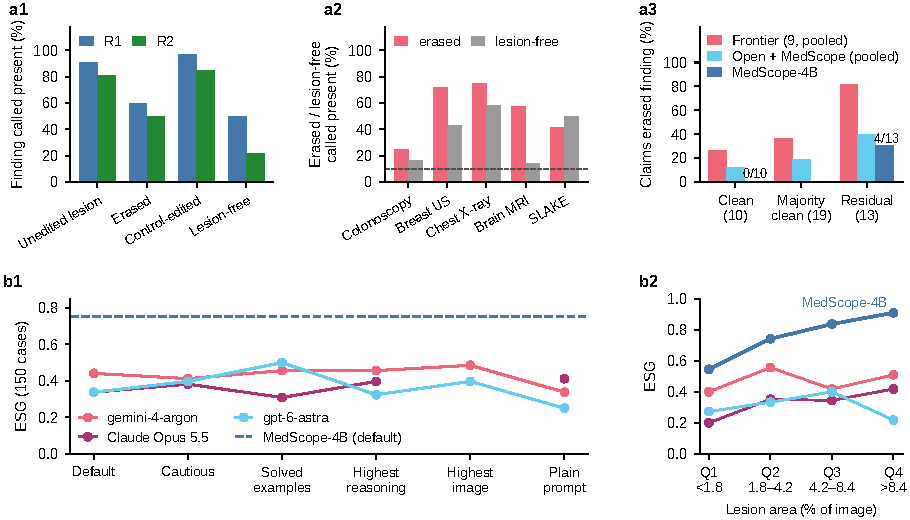
\includegraphics[width=\textwidth]{figures/fig6_readers_robustness.pdf}
\end{center}
\vspace{-0.3cm}
\caption{Readers support the erasures in colonoscopy only; the frontier models' claim rates hold across prompts and lesion sizes. (a1) Share of the $128$ main-test images ($32$ per kind) on which each blinded trainee physician (R1 internal medicine, R2 radiology; one year each) called the finding present. Edited and unedited images were not told apart (AUC $0.54$ and $0.55$). (a2) Erased and lesion-free images by source, both readers' reads pooled; the dashed line is the pre-registered $10\%$ residual criterion. Only in colonoscopy does the erased rate fall to the lesion-free rate. (a3) Stored model replies re-scored on reader-clean ($10$), majority-clean ($19$) and residual ($13$) erasures: frontier models pooled, open models and \texttt{MedScope-4B} pooled, and \texttt{MedScope-4B} alone ($0/10$ clean, $4/13$ residual; its majority-clean count was not computed). (b1) ESG of the three flagships on the same $150$ cases under six conditions (\texttt{Claude Opus 5.5} has no highest-image run); dashed: \texttt{MedScope-4B} under its default protocol. (b2) ESG by lesion-area quartile (share of the image) for \texttt{MedScope-4B} and the three flagships.}
\label{fig:readers_robustness}
\vspace{-0.2cm}
\end{figure*}

\textbf{Blinded physician reader verification.} Figure~\ref{fig:readers_robustness}a and Supplementary Table~\ref{tab:reader_study} report the results of our two-reader study on $128$ main-test images ($32$ each of $O, E, C_{\text{far}}, N$; CT denotes ``cannot tell''). First, physicians cannot distinguish edited ($E \cup C_{\text{far}}$) from unmodified ($O \cup N$) images: edit detection AUCs are $0.54$ (R1) and $0.55$ (R2) with only slight inter-reader agreement on edit status ($\text{Cohen's }\kappa = 0.10$). Second, however, readers report a clinical finding present on $35/64$ ($54.7\%$ $[41.7, 67.2]$) of pooled erased reads and $13/32$ ($40.6\%$ $[23.7, 59.4]$) of erased images by majority ($\kappa = 0.47$ on finding presence), failing our pre-specified $\le 10\%$ residual criterion. Stratified by modality (Figure~\ref{fig:readers_robustness}a2), automated LaMa erasure is \textbf{supported by the readers for colonoscopy} (finding called on $1/6$ R1 and $2/6$ R2 erased views vs.\ $2/6$ and $0/6$ on unedited lesion-free images), whereas substantial residual or secondary signs persist in breast ultrasound ($6/7 \mid 4/7$ erased vs.\ $5/7 \mid 1/7$ healthy), chest X-ray ($5/6 \mid 4/6$ vs.\ $4/6 \mid 3/6$), brain MRI ($3/7 \mid 5/7$ vs.\ $1/7 \mid 1/7$), and SLAKE ($4/6 \mid 1/6$ vs.\ $4/6 \mid 2/6$). Among the $13$ majority-residual erased images, $4$ ask the generic question \emph{``Is there an abnormality?''} (where any other abnormality in the image makes ``yes'' a correct answer), while the remaining $9$ ask lesion-specific questions. The readers did not give reasons, so why they still saw the finding on these $9$ is open; surrounding cues or incomplete mask coverage are hypotheses, not observations.

Re-scoring stored model outputs on reader-partitioned subsets (Figure~\ref{fig:readers_robustness}a3) supports the main comparison and qualifies it: across the $10$ strictly reader-clean erasures (mostly colonoscopy), the nine frontier models pooled claim the finding on $26\%$ $[10, 42]$ of cases ($30\%$, $19/63$, when conditioned on having detected the lesion on the unedited image; the pre-registered lower bound $>20\%$ was not met due to the small $n=10$ sample), $36\%$ on the $19$ majority-clean erasures, and $82\%$ on the $13$ residual erasures (whereas open-weight and MedScope models pooled claim $12\%$ on reader-clean, $19\%$ on majority-clean, and $40\%$ on residual erasures). \texttt{MedScope-4B} claims $0/10$ reader-clean erasures and $4/13$ residual erasures, while detecting $56/63$ ($88.9\%$) reader-confirmed lesions and making $0/16$ false claims on reader-confirmed healthy images. On the full main-test colonoscopy cohort ($83$ cases)---the imaging type for which the readers supported the erasures---frontier models pooled claim $45\%$ of erased polyps while detecting $96\%$ of unedited ones (vs.\ $1\%$ erased claims for \texttt{MedScope-4B}).

\textbf{External generalization and the SIIM pneumothorax failure.} Supplementary Table~\ref{tab:generalization_and_pneumo}A reports out-of-distribution generalization. On \textbf{External centres} ($169$ cases), \texttt{MedScope-4B} achieves an ESG of $0.597$ vs.\ $0.277\text{--}0.412$ for the frontier flagships (CVC-ClinicDB $0.85$, BraTS-Africa $0.71$, BUS-BRA $0.58$, but QaTa-COV19 $0.05$ because diffuse COVID-19 opacities erase poorly). On \textbf{Fresh internal} ($76$ ChestX-Det cases), \texttt{MedScope-4B} leads on ESG ($0.472$ vs.\ $0.000\text{--}0.083$) and net utility ($0.402$ vs.\ $-0.023$ to $0.219$). On \textbf{Standard VQA} ($1,051$ cases, whose training splits were seen in Stage-3 replay), \texttt{MedScope-4B} outperforms base \texttt{Qwen3.5-4B} across all three benchmarks (closed / open / overall accuracy: VQA-RAD $0.741 / 0.230 / 0.514$ vs.\ $0.657 / 0.260 / 0.481$; SLAKE $0.881 / 0.644 / 0.730$ vs.\ $0.826 / 0.424 / 0.570$; PathVQA $0.801 / 0.125 / 0.477$ vs.\ $0.545 / 0.021 / 0.293$).

However, on the confirmatory \textbf{Fresh external} cohort ($316$ cases), \texttt{MedScope-4B} trails \texttt{gemini-4-argon} in net utility ($-0.053$ vs.\ $0.310$; difference $-0.363$ $[-0.496, -0.233]$) and CCR ($0.476$ vs.\ $0.741$). By source, it is competitive on BUS-UCLM and weaker on ETIS-Larib and BraTS meningioma (Supplementary Table~\ref{tab:generalization_and_pneumo}), and it fails completely on \textbf{SIIM-ACR pneumothorax} ($\text{CCR } 0.00$, utility $-1.10$ vs.\ $0.66 / -0.06$ for \texttt{gemini-4-argon}), answering a confident \emph{``No''} (probability $\approx 1.0$) on all $48$ pneumothorax films. A post-hoc audit (Supplementary Table~\ref{tab:generalization_and_pneumo}B) shows that resolution does not explain the final model's miss: \texttt{MedScope-4B} calls pneumothorax present on $0\%$ of films both on the $256\text{-px}$ copies and on the $42$ films recovered at original resolution, whereas Stage~1 with counterfactual views reached $19\%$ and $40\%$ and Stage~2 $40\%$ at original resolution. The likely cause is training coverage: only $54$ of $\sim 7{,}000$ Stage-1 chest X-ray training views named pneumothorax, trained to answer \emph{``No''} $80\%$ of the time, from only $4$ pneumothorax lesion images, and validation held no pneumothorax lesion images, so Stage-3 replay could remove what earlier stages had without any validation penalty. As an exploratory remedy we redid Stage~3 with $150 + 150$ SIIM training patients. That model failed the pre-set selection rule (validation healthy-image claims $10.0\%$ vs.\ $7.7\%$, limit $+2$ points), so \texttt{MedScope-4B} remains the reported model. Tested anyway on $200$ new SIIM patients ($100$ with and $100$ without pneumothorax), it found $27\%$ of pneumothorax films (\texttt{MedScope-4B}: $0\%$) and called no healthy film positive, and on the main test it kept ESG $0.804$ and erased-lesion claims $5.5\%$ ($0.758$ and $9.6\%$ for \texttt{MedScope-4B}). Training coverage therefore explains part of the miss, but detection stays far below \texttt{gemini-4-argon}'s $69\%$.

\subsection{Checks Added After an External Review}
\label{subsec:exp_review}
An external review asked whether the remaining limit is a property of the frozen encoder, how the framework compares with CORAL \citep{zafar2026coral}, and whether the abstention ceiling can be measured. Four checks were pre-registered before they ran (repository document \texttt{REVIEW\_EXPERIMENTS.md}); the two training arms were screened on the validation dev set only, one seed each (Supplementary Table~\ref{tab:review_checks}).

\textbf{A CORAL-style comparator.} CORAL's weights are not public, so we added its training signal to our pipeline: the replay-only control continuation plus one term asking the answer to change when the image is swapped for the most similar lesion-free training image of another patient (CLIP retrieval, $2{,}603$ of $2{,}739$ cases). Against the control, held-out TELEA ESG changed by $-0.028$ $[-0.073, 0.017]$ and LaMa ESG by $+0.011$ $[-0.022, 0.050]$; the pre-registered rule (TELEA ESG $+0.03$) was not met. During training the model already rejected the swapped image by about $26$ nats, against a margin of $2$, so the term rarely acted: a whole-image swap is too easy a contrast to teach lesion-level evidence.

\textbf{Vision adapters with layer-wise decay.} The stage-1 recipe with LoRA also on the vision encoder and projector, the top block at a tenth of the language model's learning rate and each lower block at $0.9$ times the one above, found $+0.017$ $[-0.034, 0.067]$ more unedited lesions than the frozen-encoder recipe; the rule asked for $+0.03$ and was not met. Its ESG rose by $+0.061$ $[-0.011, 0.134]$ (LaMa) and $+0.034$ $[-0.028, 0.101]$ (TELEA) and its lesion-free claims fell by $0.075$ $[-0.150, 0.000]$, all within noise for one seed, while its denial of intact lesions after a TELEA ring edit rose by $+0.075$ $[0.030, 0.128]$. Gently adapting the encoder did not make the model see more lesions.

\textbf{Is the limit this encoder?} The same linear probe on four frozen image encoders separates an erasure from the control edit of the same case (main-test views) as follows: Qwen3.5-4B's own encoder $0.86$, $0.86$ and $0.80$ AUC on LaMa, TELEA and Stable Diffusion views (whole image; $0.90$, $0.87$ and $0.84$ on a lesion-centred crop); BiomedCLIP $0.01$ to $0.06$ lower (crop intervals include zero); DINOv2 $0.07$ to $0.17$ lower; RAD-DINO $0.13$ to $0.23$ lower. No alternative met the pre-registered reading (better by $0.05$ with the interval above zero), so we find no evidence that another frozen encoder holds more of this separation. Qwen's encoder is also the most edit-sensitive: it separates a control-edited image from the unedited one at $0.61$--$0.75$ AUC (whole image), so an ``edited means absent'' shortcut is available to the model, which is what the matched control is for.

\textbf{The abstention ceiling, measured.} An out-of-sample linear probe's hard call is one fixed event, so its true-positive minus false-positive rate is a lower bound on the total-variation distance in Proposition~1. For the stage-1 recipe on the validation dev set, the bound between erased and ring-edited views at the best layer is $0.64$--$0.67$ on LaMa views, against the model's own denial gap of $0.65$, and $0.49$--$0.62$ on TELEA views, against $0.64$: the answers use all the separation a linear read-out finds (no read-out gap). For the untrained base model the bound is $0.55$--$0.57$ (LaMa) and $0.47$--$0.52$ (TELEA), while its answers' denial gap is only $0.02$ and $0.13$ ($54$ cases with answers on both views). The base model's hidden states already hold the separation that its answers ignore; counterfactual training closes that read-out gap, and the remaining limit is what the hidden states hold.
%%%%%%%%% EXPERIMENTS %%%%%%%%%

\section{Discussion and Limitations}
\label{sec:discussion}
%%%%%%%%% DISCUSSION %%%%%%%%%

\subsection{What Counterfactual Evaluation Can and Cannot Certify}
\label{subsec:disc_certify}
For focal mucosal lesions in colonoscopy, automated inpainting with LaMa reduces physician finding calls to the level of unedited healthy tissue ($1/6$ and $2/6$ vs.\ $2/6$ and $0/6$), supporting that the visual evidence is removed. In this reader-validated regime, nine frontier VLMs still claim $45\%$ of $83$ erased polyps while detecting $96\%$ of unedited ones---and claim $30\%$ of reader-clean erasures whose unedited counterpart they correctly detected---evidence that frontier models often answer such questions from the question rather than the pixels.

On the other hand, across all sources (colonoscopy included), physicians still call a finding present on $54.7\%$ of pooled erased reads ($40.6\%$ of erased images by majority), even though they cannot tell edited from unedited images ($\text{AUC } 0.54\text{--}0.55$); most of these residual calls fall outside colonoscopy, and in diffuse disease such as COVID-19 opacities erasure works poorly (QaTa-COV19 $\text{ESG } 0.05$). The readers did not record what they saw, so the cause (secondary signs outside the mask, or incomplete mask coverage) remains a hypothesis. Because counterfactual training labels every erased view ``absent'', training on unverified erasures outside colonoscopy may teach a model to discount whatever residual evidence remains (though \texttt{MedScope-4B} still claims $4/13$ residual erasures vs.\ $0/10$ reader-clean ones). Furthermore, held-out editing tools introduce generator-specific failure modes: TELEA's smooth PDE patches trigger $12.9\%$ false denials on intact lesions, whereas $41/45$ false claims on Stable Diffusion erasures point at the inpainted site, which may hold residual or regenerated tissue (these erasures were not reader-checked). Consequently, unverified automated ESG cannot be treated as a pure measure of hallucination in isolation; counterfactual benchmarks must pair target erasures with symmetric controls, held-out generators, and physician reader checks.

\subsection{Implications of the Pre-Registered Negative Map and the Perception Limit}
\label{subsec:disc_negative_map}
Every intervention that appeared to improve utility or reduce erased-lesion claims did so by moving the operating threshold, and the probes are consistent with this: the read-out gap between hidden representations and behavioral answers on held-out TELEA edits is at most $+0.028$ AUROC, and the untrained \texttt{Qwen3.5-4B} base model's hidden states already separate erased from intact lesions nearly as well as the trained recipe's ($0.83\text{--}0.87$ vs.\ $0.85\text{--}0.90$). The answers therefore do not leave usable separation unread, and the remaining limit is \textbf{perception}: $15\%\text{--}20\%$ of real lesions are missed on unedited images, and every miss also lowers ESG. This is the perception of a frozen, general-domain encoder: adapting it with low-rank adapters at two learning rates did not improve it, but full fine-tuning was not tested. Adding layer-wise learning-rate decay did not improve it either, and three other frozen encoders, including the medical BiomedCLIP, hold no more of this separation than Qwen's own (Section~\ref{subsec:exp_review}).

\textbf{Where \texttt{MedScope-4B} fails.} Its errors concentrate in five places: the smallest lesions (ESG $0.545$ and $18.2\%$ erased claims in the smallest area quartile); chest X-ray and SLAKE CT/MRI (ESG $0.51$ and $0.47$, against $0.95$ in colonoscopy); diffuse findings, which do not erase cleanly (QaTa-COV19 ESG $0.05$); rare findings absent from training and validation (pneumothorax, $0/48$); and denial of intact lesions after an unfamiliar edit near them, concentrated in chest X-rays ($12/17$ of the TELEA ring denials).

\textbf{Limitations.} Beyond residual findings in automated erasures and the perception limit, our study has five limitations: (1) as exposed by the $0/48$ SIIM pneumothorax failure, counterfactual training on a skewed label distribution ($80\%$ \emph{``No''} on $54$ pneumothorax queries and only $4$ positive images) followed by Stage-3 replay can remove sensitivity to a rare finding without triggering the selection rule when validation holds no positive image of it; adding SIIM training patients recovers only part of it ($27\%$, exploratory); (2) our clinical cost matrix was fixed prior to experimentation rather than elicited from practicing clinicians for specific workflows; (3) the physician reader study, while blinded and stratified, covers a modest sample ($128$ views, yielding $10$ strictly reader-clean erasures) with two trainee physicians (internal medicine and radiology, $1\text{ year}$ each) and did not evaluate Stable Diffusion erasures; and (4) \texttt{MedScope-4B} exhibits poorer verbalized confidence calibration for selective prediction ($\text{AURC } 0.065$) than frontier models ($0.020\text{--}0.033$), and its raw single-turn log-odds are not a valid confidence score across cases, because replies with box coordinates are $\sim 11\text{ nats}$ less likely than short absent replies on every image; and (5) demographic and acquisition details are not compiled: most public sources release none per image, so performance by age, sex or scanner is not reported.
%%%%%%%%% DISCUSSION %%%%%%%%%

\section{Conclusion}
\label{sec:conclusion}
%%%%%%%%% CONCLUSION %%%%%%%%%
We presented a Counterfactual Evidence Framework that measures whether medical vision--language agents answer closed clinical questions from the image or from the question, with matched control edits, held-out editing tools, threshold-free metrics, an abstention ceiling, blinded physician readers and hidden-state probes. Three conclusions follow. First, nine frontier VLMs claim $41.1\%$ to $61.6\%$ of erased findings across diverse prompting regimes---including $45\%$ in reader-validated colonoscopy---whereas training a 4B reference agent (\texttt{MedScope-4B}) on automatically constructed counterfactual trajectories reduces erased claims to $9.6\%$ and raises ESG to $0.758$. Second, across twelve pre-registered post-training and multi-agent interventions and $270$ decision policies, apparent improvements over counterfactual SFT stem from shifting the answer or abstention threshold rather than improving visual discrimination, and representation probes find no read-out gap, pointing to the perception of this frozen-encoder model as the remaining limit. Third, our physician reader study and external pneumothorax failure audit indicate that counterfactual evaluation requires verifying automated erasures for residual clinical signs and ensuring positive validation coverage across all target pathologies.

\section*{Code and Data Availability}
All pre-registration documents, source code, quality-control scripts, the reader-study interface and the stored per-view outputs of every model (frontier APIs evaluated 31 October 2026 under provider default settings) are at \url{https://github.com/bhaskargurram-ai/medscope}. The numeric tables numbered S, the reporting checklist and the pre-registration details are in the online supplement in the same repository (\texttt{paper/jbhi/supplement.pdf}). All images are public; the sources are cited in Section~\ref{subsec:exp_setup} and the exact copies used are listed in the supplement.

\bibliography{\jobname}
\bibliographystyle{IEEEtranN-doi}

%%%%%%%%% Appendix %%%%%%%%%
\newpage
\end{document}
